
\documentclass[11pt,a4paper]{article}
% \renewcommand{\baselinestretch}{2}

\input{psfig}
\textwidth 15.6truecm
\textheight 23truecm
\hoffset -1.5truecm
\voffset -1.5truecm
 
\title{{\huge \bf Entropy Measure from Noise Modeling: theory and applications}}

\bigskip
\bigskip
\bigskip

\author{ $ $ \\  
$ $ \\ 
J.-L. Starck \\ [12pt]
$ $ \\ 
DAPNIA/SEI-SAP, CEA/SACLAY, F-91191 Gif sur Yvette Cedex}

\bigskip
\bigskip
\bigskip


\date{$ $ \\ [12pt]
January 1998 }


\begin{document}
\maketitle
 
\abstract{ $ $ \\ [12pt]
We present in this report a new way to measure the information
in a signal, based on noise modeling. We show how the use of such 
an entropy-related measure is helpfull for filtering and deconvolution.
A set of examples illustrates the results.  It can also be used for tracking
the presence of signal in a noisy data set.}


\newpage
\tableofcontents
\newpage


\chapter{Data on the Sphere}
\label{ch_intro}

\section{Introduction}

In a number of areas of scientific activity, data is gathered which naturally maps to the sphere. For instance, remote sensing of the 
Earth's surface and atmosphere,\emph{e.g.} with POLDER\footnote{\emph{http://polder.cnes.fr}}, generates spherical data maps which are 
crucial for global and local geophysical studies such as understanding climate change, geodynamics or monitoring human-environment 
interactions. More examples can be found in medical imaging or computer graphics. In astronomy and astrophysics, recent and upcoming 
ground based and satellite borne experiments such as WMAP\footnote{\emph{http://map.gsfc.nasa.gov}} or Planck-Surveyor\footnote{\emph{http://astro.estec.esa.nl/Planck}} 
for the observation of the Cosmic Microwave Background radiation field over the whole celestial sphere, have and will produce full-sky 
maps in a wide range of wavelengths. These maps are necessarily digitized and hence distributed as a finite set of pixel values on some 
grid. The properties of this grid will affect the subsequent analysis of the data, and a good choice will make standard computations, 
such as the spherical harmonics transform, much faster and accurate. Considerable work has been dedicated to the development of 
pixelization schemes on the sphere. In particular, Healpix\cite{healpix} is a sampling scheme which has some attractive geometrical 
features profitably used in this spherical data analysis software package. \\

Processing spherical data maps requires specific tools or somehow adapting traditional methods used on flat images to the spherical 
topology, such as multiscale transforms for image processing. Among these, Wavelets and related representations are by now successfully 
used in all areas of signal and image processing. Their recent inclusion in JPEG 2000 -- the new still-picture compression standard -- 
is an illustration of this lasting and significant impact. Wavelets are also very popular tools in astronomy \cite{starck:book02} which 
have led to very impressive results in denoising and detection applications. For instance, both the Chandra and the XMM data centers 
use wavelets for the detection of extended sources in X-ray images. For denoising and deconvolution, wavelets have also demonstrated 
how powerful they are for discriminating signal from noise \cite{starck:sta02_2}. In cosmology, wavelets have been used in many studies 
such as for analyzing the spatial distribution of galaxies \cite{astro:slezak93,astro:escalera95,starck:sta05,starck:martinez05}, 
determining the topology of the universe \cite{astro:rocha04}, detecting non-Gaussianity in the CMB maps \cite{gauss:aghanim99,gauss:barreiro01_1,wave:vielva04,starck:sta03_1},
reconstructing the primordial power spectrum \cite{astro:pia03}, measuring the galaxy power spectrum \cite{astro:fang00} or reconstructing 
weak lensing mass maps \cite{starck:sta05b}. It has also been shown that noise is a problem of major concern for N-body simulations of 
structure formation in the early Universe and that using wavelets for removing noise from N-body simulations is equivalent to simulations 
with two orders of magnitude more particles \cite{rest:romeo03,rest:romeo04}. 

Wavelets owe part of their success to their ability for sparse approximation of point singularities. However they are not as good at detecting 
highly anisotropic features such as curvilinear singularities in images. This is where other multiscale systems such as Ridgelets \cite{cur:candes99_1} 
and Curvelets \cite{cur:donoho99,starck:sta01_3}, which exhibit high directional sensitivity and are highly anisotropic, come into play. Digital 
implementations of both ridgelet and curvelet transforms for image denoising are described in \cite{starck:sta01_3}. Inspired by the successes 
of \emph{Euclidean} wavelets, ridgelets and curvelets, this package provides implementations of new multiscale decompositions for spherical images 
namely the isotropic undecimated wavelet transform, the ridgelet transform and the curvelet transform each of which is invertible.

\section{Pixelization}

Despite the apparent simplicity of the sphere, deriving numerical schemes on the sphere is not a trivial task. A major difficulty encountered 
in the design of numerical methods on the sphere is that of pixelization: there is no obvious way in which to reconcile the requirements 
for a \emph{maximally} uniform sampling and for an exact and invertible computation of the spherical harmonics decomposition of band-limited 
functions \cite{healpix,icosahedron}. Also, the sampling strategy determines largely the achievable algorithmic complexity of these computations. 
Several sampling schemes have been proposed recently such as Tegmark's Icosahedron \cite{icosahedron}, the Igloo \cite{igloo} or Healpix \cite{healpix} 
methods which tend to favor approximate uniformity among other properties. The Glesp \cite{glesp} pixelization was developed with a strong 
focus on the accuracy of the spherical harmonics transform. 

\subsection*{Healpix}

The Healpix representation is a curvilinear hierarchical partition of the sphere into quadrilateral pixels of exactly equal area but with 
varying shape. The base resolution divides the sphere into 12 quadrilateral faces of equal area placed on three rings around the poles 
and equator. Each face is subsequently divided into $nside^{2}$ pixels following a quadrilateral multiscale tree structure. The pixel 
centers are located on iso-latitude rings, and pixels from the same ring are equispaced in azimuth. This is critical for computational 
speed of all operations involving the evaluation of spherical harmonics transforms, including standard numerical analysis operations such 
as convolutions, power spectrum estimation\ldots \\

\begin{figure}
\centering
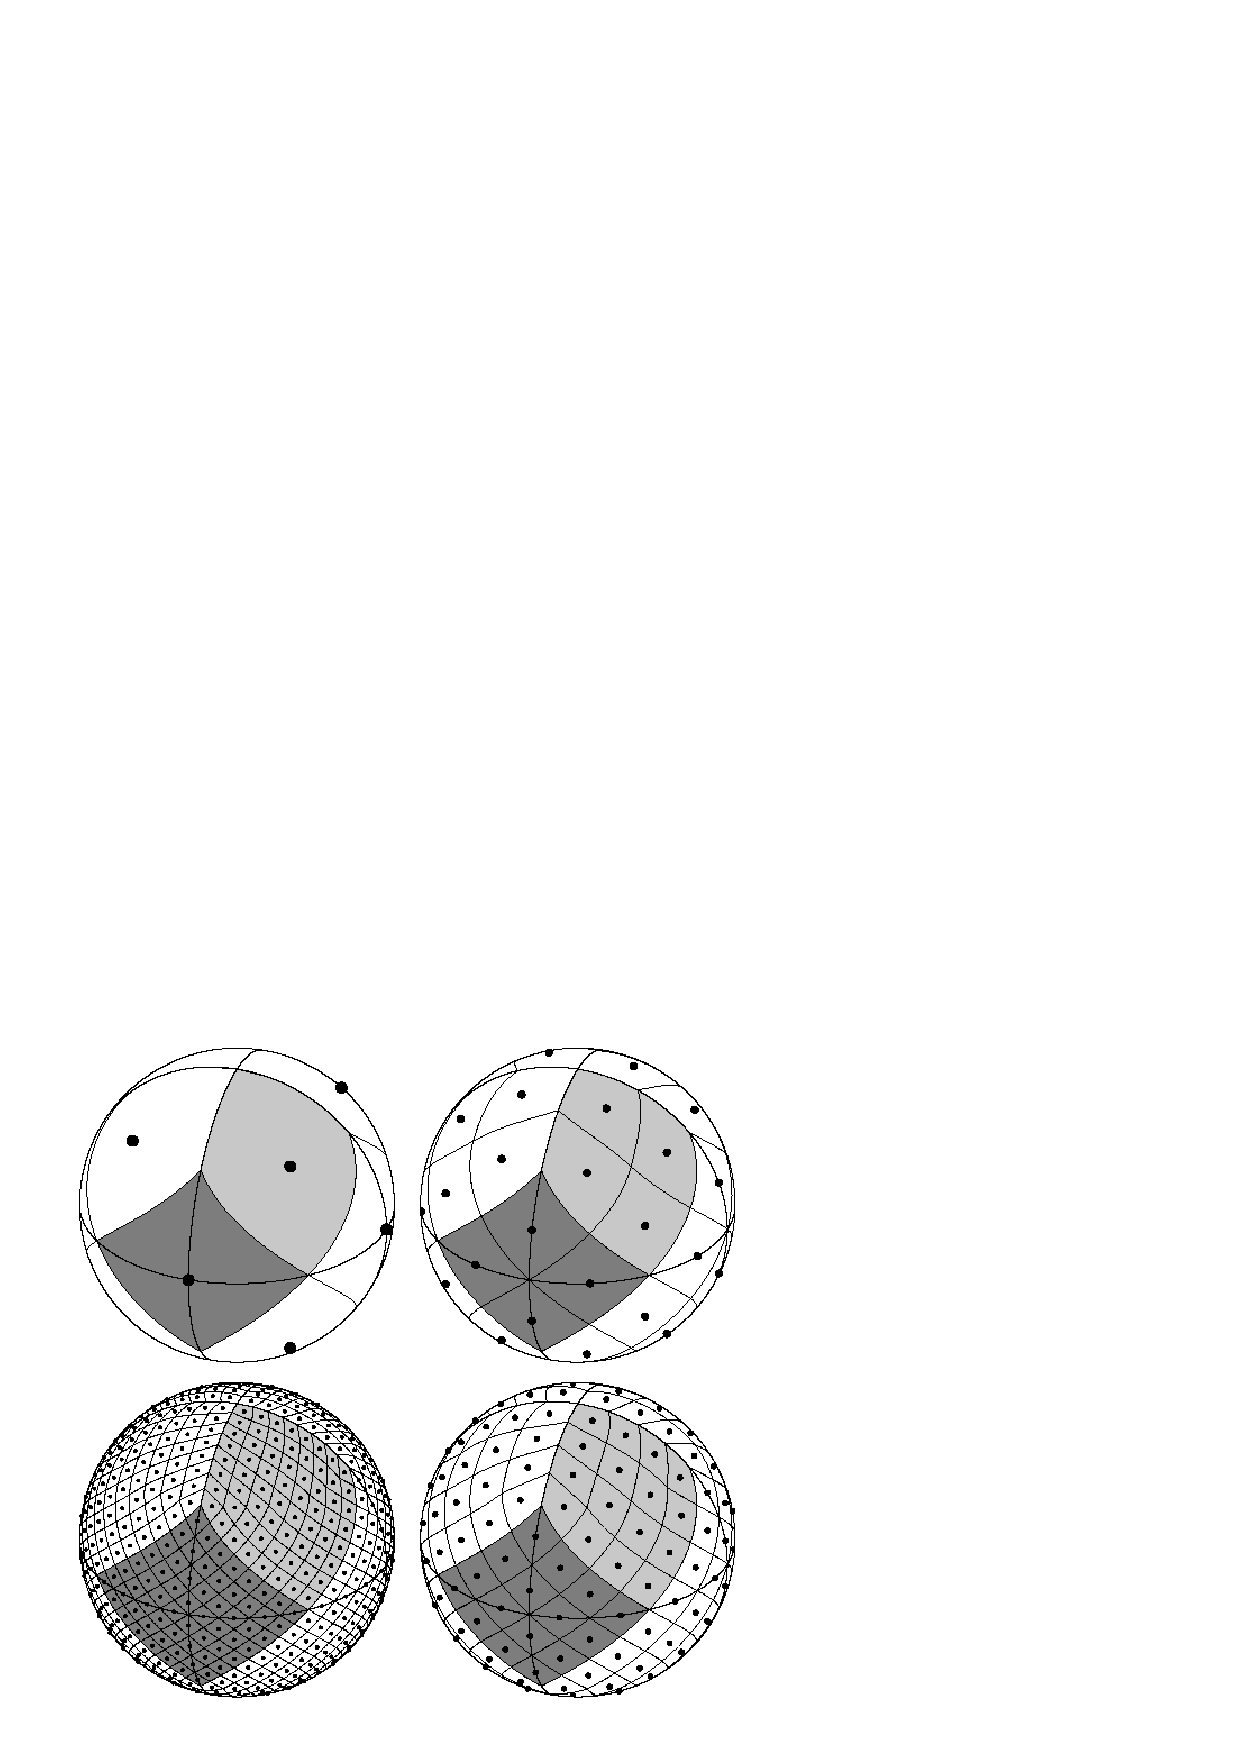
\includegraphics{pixelhealpix}
\caption{The Healpix sampling grid.}
\label{pixelhealpix}
\end{figure}

An important geometrical feature of the Healpix sampling grid is the hierarchical quadrilateral tree structure. This defines a \emph{natural} 
one-to-one mapping of the sphere sampled according to the Healpix grid, into twelve \emph{flat} images, on all scales. It is then easy to 
partition a spherical map using Healpix into quadrilateral blocks of a specified size. One first extracts the twelve base-resolution faces, 
and each face is then decomposed into overlapping blocks of the specified size. This decomposition into blocks is an essential step of the 
traditional \emph{flat} 2D curvelet transform. Based on the reversible warping of the sphere into a set of flat images made possible by the 
Healpix sampling grid, the ridgelet and curvelet transforms can be extended to the sphere. 

With the decomposition into blocks described above, there is no overlapping between neighboring blocks belonging to different base-resolution faces. 
This may result for instance in blocking effects in denoising experiments \emph{via} non linear filtering. It is possible to overcome this difficulty 
in some sense by working simultaneously with various rotations of the data with respect to the sampling grid. This will average out undesirable 
effects at edges between base resolution faces. 

\section{Multiscale methods on the sphere}

\subsection{Wavelets on the sphere}

In the last years, several wavelet transforms on the sphere have been proposed. Schr{\"o}der and Sweldens \cite{wave:sweldens95a} have developed 
an orthogonal wavelet transform on the sphere based on the Haar wavelet function which then suffers from the poor properties of the Haar function 
and the problems inherent to the orthogonal decomposition. A few papers describe continuous wavelet transforms on the sphere \cite{wave:antoine99,wave:tenerio99,wave:cayon01,wave:holschneider96}. 
An application to the detection of non-Gaussianity in the CMB radiation using the stereographic Mexican hat wavelet is reported in \cite{wave:vielva04}. 
These methods have been extended to directional wavelet transforms \cite{wave:antoine01,wave:hobson04,wave:wiaux}. Although profitable for data 
analysis, these continuous transforms lack an inverse transform and hence are clearly not suitable for restoration purposes. The algorithm proposed 
by Freeden and Maier\cite{freeden97,freeden98}, based on the Spherical Harmonic Decomposition, is to our knowledge the only one to have an inverse transform.\\  

A very popular wavelet algorithm in astrophysical applications is the so-called ``\emph{\`a trous} algorithm'' (a better name would be the 
``isotropic undecimated wavelet transform'' ), which possesses the following features: i) it is isotropic, ii) it is undecimated, iii) it uses 
an order three Box-Spline as scaling function. The isotropy of the wavelet function makes this decomposition optimal for the detection of 
isotropic objects. The non decimation makes the decomposition redundant (the number of coefficients in the decomposition is equal to the number 
of samples in the data multiplied by the number of scales) and allows us to avoid Gibbs aliasing after reconstruction in image restoration 
applications, as generally occurs with orthogonal or bi-orthogonal wavelet transforms. The choice of a $B_3$-spline is motivated by the fact 
that we want an analyzing function close to a Gaussian, but verifying the dilation equation, which is required in order to have a fast transformation. 
Finally the last property of this algorithm is to provide a very straightforward reconstruction. Indeed, the sum of all the wavelet scales and 
of the coarsest resolution image reproduces exactly the original image. \\

The \mrs package offers an implementation of a new isotropic wavelet transform on the sphere. Its properties are similar to those of the \emph{\`a trous} 
algorithm and therefore should be very useful for data denoising and deconvolution. This algorithm, described in chapter~\ref{ch_mms}, is directly derived
from the FFT-based wavelet transform proposed in\cite{starck:sta94_3} for aperture synthesis image restoration. It is relatively close to the Freeden and 
Maier \cite{freeden98} method, except that the reconstruction process is as straightforward as in the \emph{\`a trous} algorithm (i.e. the sum of the scales 
reproduces the original data). This new wavelet transform can also be easily extended to a pyramidal wavelet transform, which may be very important for 
larger data sets such such as from the future Planck experiment.

\subsection{Ridgelets and Curvelets on the sphere}
 
When analyzing data which contains anisotropic features, wavelets are no longer optimal. This has motivated the development of new multiscale 
decompositions such as the ridgelet and the curvelet transforms \cite{cur:donoho99,starck:sta01_3}. Among possible applications of those data 
analysis methods, it was shown in Starck et al. \cite*{starck:sta03_1} that the \emph{flat} curvelet transform could be useful for the detection 
of non Gaussianity in \emph{flat} patches of CMB data, and also to discriminate among different causes of non Gaussianity. 

In this area, further insight will come from the analysis of full-sky data mapped to the sphere thus requiring the development of a curvelet 
transform on the sphere. The \mrs package offers an implementation of ridgelet and curvelet transforms for spherical maps. Those implementations 
are derived as extensions of the digital ridgelet and curvelet transforms described in \cite{starck:sta01_3}. The implemented undecimated isotropic 
wavelet transform on the sphere and the specific geometry of the Healpix sampling grid are important components of the present implementation of 
curvelets on the sphere. \\
 
Further motivation for developing these new multiscale methods on the sphere follows from the results obtained in different data processing applications. 
As described in chapter\ref{ch_restore}, the \mrs package provides the necessary tools to experiment with these new spherical multiscale transforms in 
denoising applications, for instance using the Combined Filtering Method, which allows us to filter data on the sphere using both the Wavelet and the 
Curvelet transforms. The analysis of multichannel data mapped to the sphere, a problem encountered for instance in the processing of WMAP and Planck 
observations, is another issue that is shown to benefit from the developed multiscale representations on the sphere. This is reported in chapter~\ref{ch_mrs_ica} 
which is dedicated to describing some methods in multichannel data analysis extended to spherical maps which are implemented in the \mrs package.  
 
\section{Processing of polarized datas on the sphere}

Polarized maps are a special kind of multi-dimentionnal datas with strong links between their components. The polarization is of great importance 
in physics or astrophysics as it's analysis denotes fundamentals characteristics of the observed object or phenomenum. An example of great interest 
is today the cosmic microwave background \cite{starck}.

The statistical analysis of the slight intensity fluctuations in the primordial cosmic microwave background radiation field, for which evidence was 
found for the first time in the early 1990's in the observations made by COBE~\cite{gauss:smoot92}, is a major issue in modern cosmology as these 
are strongly related to the cosmological scenarios describing the properties and evolution of our Universe. In the Big Bang model, the observed CMB 
anisotropies are an imprint of primordial fluctuations in baryon-photon density from a time when the temperature of the Universe was high enough above 
3000~K for matter and radiation to be tightly coupled. At that time, the attraction of gravity and the repulsive radiation pressure were opposed, thus 
generating so-called acoustic oscillations in the baryon-photon fluid, causing peaks and troughs to appear in the power spectrum of the spatial anisotropies 
of the CMB. With the Universe cooling down as it expanded, matter and radiation finally decoupled. Photons were set free in a nearly transparent Universe, 
while the density fluctuations collapsed under the effect of gravity into large scale structures such as galaxies or clusters of galaxies. Due to the 
expansion of the Universe, the CMB photons are now observed in the microwave range but are still distributed according to an almost perfect black body 
emission law. Another major result was the measurement of the polarization state and anisotropies of the CMB radiation field by DASI~\cite{dasi}. 
Only a fraction of the total CMB radiation is polarized so that extremely sensitive instruments are needed. Polarization of the CMB radiation is a 
consequence of the Thomson scattering of photons on electrons. But for the outgoing population of photons to be polarized, the radiation incident on 
the scatterer needs to be anisotropic and have a quadrupole moment. The statistics of the CMB polarization anisotropies are also a source of information 
for cosmology. Inference of cosmological parameters from the joint statistics of the CMB anisotropies should benefit from both the complementarity and 
the redundancy of the information carried by the additional measurement of CMB polarization. Hence the full-sky maps with unprecedented sensitivity and 
angular resolution of both temperature and polarization anisotropies of the CMB to be delivered by the upcoming Planck Surveyor satellite experiment are 
awaited with excitement.

\subsection{Orthogonal representation of polarized datas}
\label{sec:polar}

\begin{figure*}[htb]
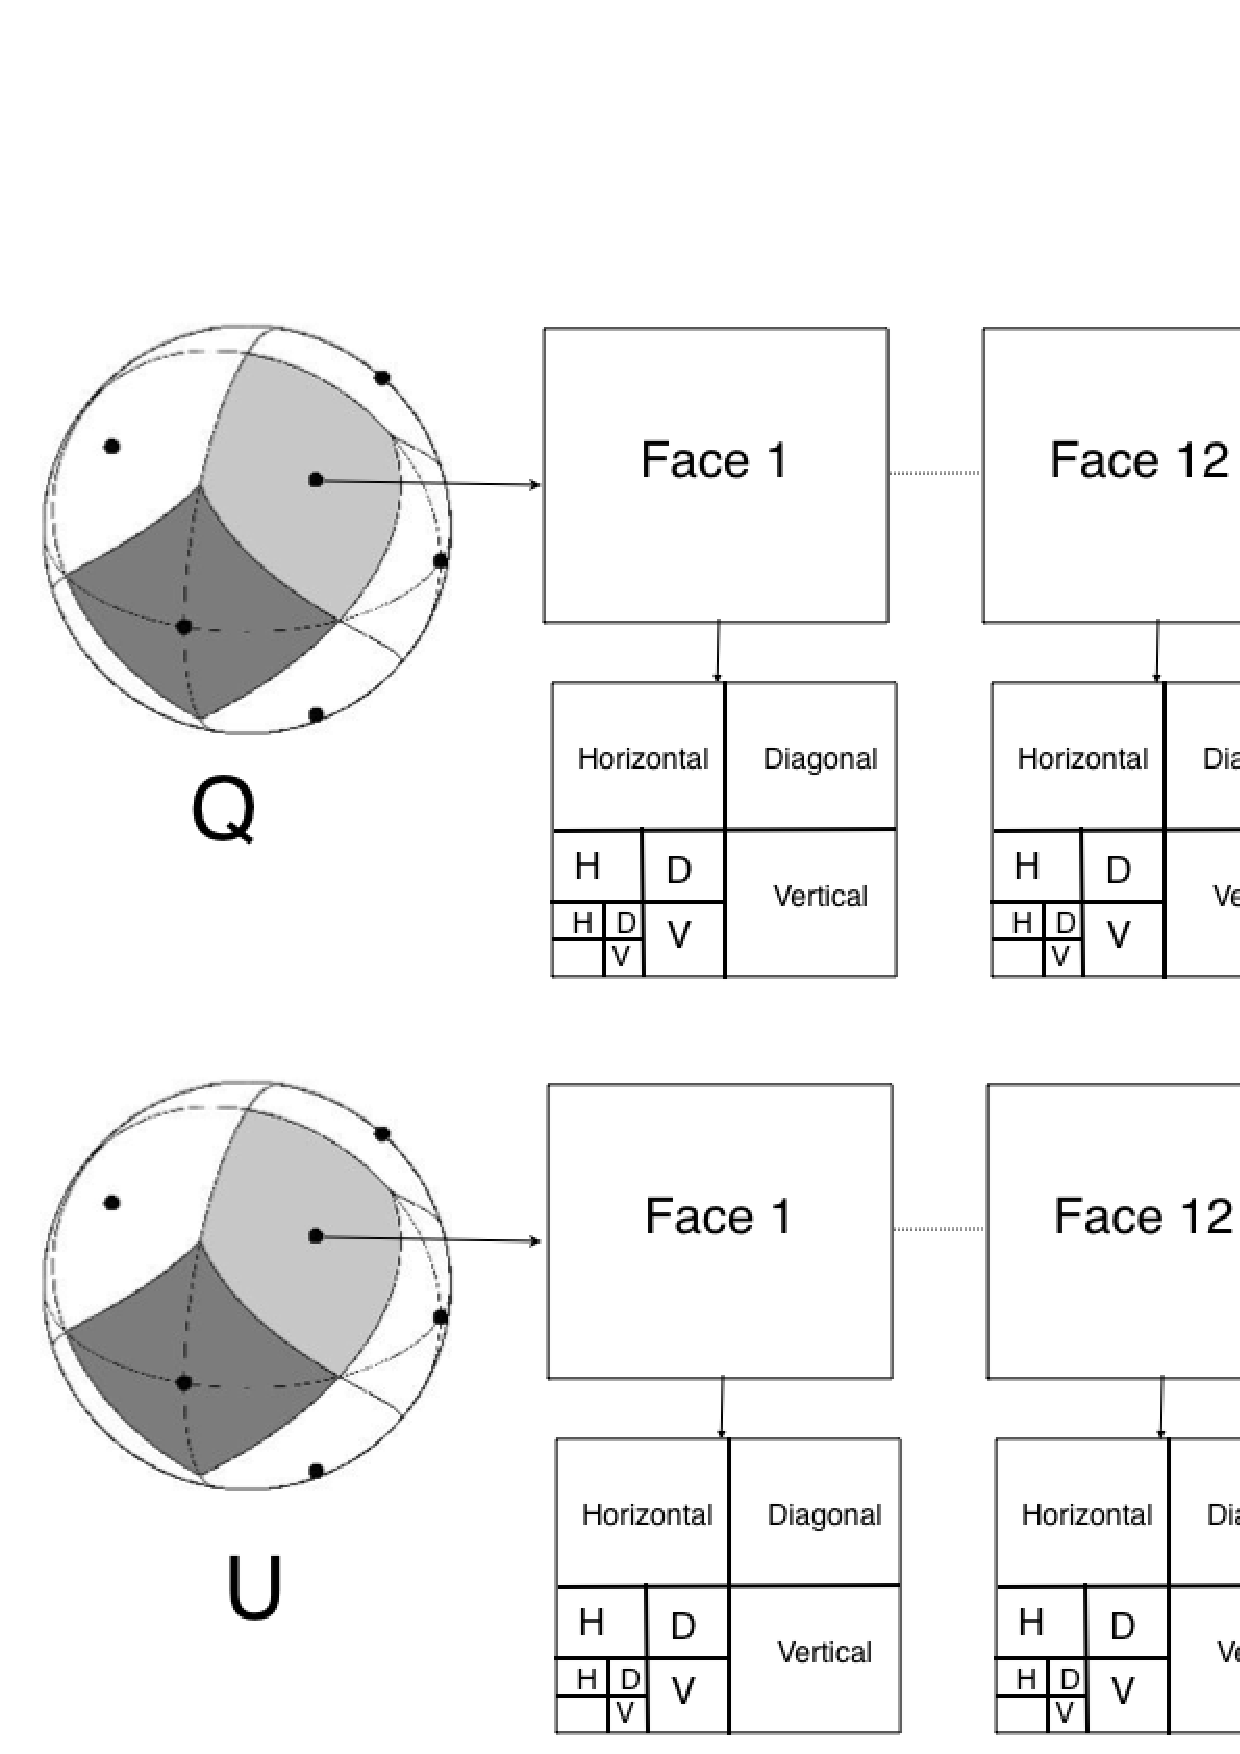
\includegraphics[width=\textwidth]{fig_pola_qu_owt_trans.pdf}
\caption{Q-U orthogonal Wavelet Transform.}
\label{fig_qu_owt_trans}
\end{figure*}
Full-sky CMB polarization data, as expected from the upcoming Planck experiment, consists of measurements of the Stokes parameters so that in addition 
to the temperature $T$ map, $Q$ and $U$ maps are given as well. The fourth Stokes parameter commonly denoted $V$ is a measure of circular polarization. 
In the case of CMB which is not expected to have circularly polarized anisotropies, $V$ vanishes. The former three quantities, $T$, $Q$ and $U$ then 
fully describe the linear polarization state of the CMB radiation incident along some radial line of sight : $T$ is the total incoming intensity, $Q$ is 
the difference between the intensities transmitted by two perfect orthogonal polarizers the directions of which define a reference frame in the tangent 
plane, and $U$ is the same as $Q$ but with polarizers rotated 45 degrees in that tangent plane. Clearly, $Q$ and $U$ are not invariant through a rotation 
of angle $\phi$ of the local reference frame around the line of sight. In fact, it is easily shown that~:
\begin{eqnarray}
Q ' = & \cos (2 \phi) Q + \sin(2 \phi) U \\ \nonumber
U ' = & \cos (2 \phi) U - \sin(2 \phi) Q 
\end{eqnarray}
which can also be written $Q' \pm i U' = e^{\mp i\phi} ( Q \pm i U )$ which by definition expresses the fact that the quantities $Q \pm i U$ are 
spin-2 fields on the sphere. The suitable generalization of the Fourier representation for such fields is the spin-2 spherical harmonics basis 
denoted $_{\pm 2}Y_{\ell m}$, in which we can expand~: 
\begin{eqnarray}\label{QU}
Q \pm i U  = \sum_{\ell, m} { _{\pm 2}a_{\ell m}} {_{\pm 2}Y_{\ell m} }
\end{eqnarray}

It is convenient~\cite{zalda} to introduce the two quantities denoted $E$ and $B$ which are defined on the sphere by~:
\begin{eqnarray}\label{EB}
E = & \sum_{\ell, m} a_{\ell m} ^E Y_{\ell m} = \sum_{\ell, m} - \frac{1}{2} ( {_{ 2}a_{\ell m}} + {_{- 2}a_{\ell m}} ) Y_{\ell m} \\ \nonumber
B = & \sum_{\ell, m} a_{\ell m} ^B Y_{\ell m} = \sum_{\ell, m} i \frac{1}{2} ( {_{ 2}a_{\ell m}} - {_{- 2}a_{\ell m}} ) Y_{\ell m} 
\end{eqnarray}

\subsection{Multiscale transform on the sphere for polarized datas}

Inprovements in the second version of the \mrs package includes extension of the 1D multiscale transforms to the case of polarized maps with 
the three fields $T$, $Q$ and $U$ (or the fields $T$, $E$ and $B$). The easiest way to build a multiscale transform for polarized data is to 
use the Healpix\footnote{http://healpix.jpl.nasa.gov} representation \cite{pixel:healpix}, and to apply a bi-orthogonal wavelet transform 
on each face of the Healpix map, separately for $Q$ and $U$. Fig.~\ref{fig_qu_owt_trans} shows the flow-graph of this Q-U orthogonal wavelet 
transform (QU-OWT). Most of the algorithms included in \mrs for the processing of 1D images know have a version for polarized maps.

% \clearpage
% \newpage




\section{Entropy from Noise Modeling}
\index{multiscale entropy}
\subsection{Information and wavelet coefficient}
In the case of signal restoration, the noise is the main problem. This 
means that we should not consider the probability of appearance of 
a pixel value in an image, but rather its probability of being due to the
signal (or to the noise). 
If we consider a variable $x$ which follows a probability distribution 
$p(x)$, we
can define the information in $x$ by $- \ln(p(x))$, and a signal $S$ can
be considered as a set of individual variables $x_k$ (pixels), each of which 
follows the same probability distribution. 
Then the information contained in the data 
can be measured by $- \sum_{k=1}^N \ln(p(x_k))$. If $X$ follows a Gaussian 
distribution with zero mean, we have
\begin{eqnarray}
H(X) = \sum_{k=1}^N \frac{x_k^2}{2 \sigma^2} + \rm{Cst}
\end{eqnarray}
The energy gives a good measurement of information. But many of the required
criteria are not fulfilled by using such an entropy (correlation between 
pixels, background-independence, etc.). It seems difficult to derive
a good probability distribution from the pixel values which fulfill the 
entropy requirements.

This is not so for transformed data, especially when using  
the wavelet transform. 
This has  already been done, in fact,
for finding threshold levels in filtering 
methods by means of wavelet coefficient thresholding 
\cite{starck:sta95_1,rest:moulin99,rest:donoho93_1,rest:krim92,wave:chipman97,wave:amato97}. 
Thus we must introduce the concept of multiresolution into our entropy.
We will now consider that the information contained in some dataset
is the sum of the information at different resolution levels $j$.
The wavelet transform $W$ of a signal by a fast algorithm contains a set
of coefficients $w_{j,k}$ ($j$ being the scale index), and a set 
of coefficients $c_{k}$ representing the signal at a very low resolution 
(see \cite{ima:mallat98,starck:book98} for more information about the
wavelet transform). If the number of scales is enough large,
we can assume that the coefficients $c_{k}$ furnish information only
about the background, and not on the signal of interest. The entropy of $X$
must be measured only from the
wavelet coefficients $w_{j,k}$.

% Choosing the \`a trous wavelet transform (see \cite{starck:sta95_1} 
% for a description of this wavelet transform algorithm), a signal $X$ can 
% be represented by:
% \begin{eqnarray}
% X_k = \sum_{j=1}^{l} w_{j,k} + c_{l,k}
% \end{eqnarray}
% where $k$ is the pixel index, $w_j$ are the wavelet coefficients of $S$, 
% $j$ the resolution
% level, and $c_l$ is smoothed version of $S$. 
Due to the properties of
the wavelet transform, the set $w_{j}$ for all $j$ has a zero mean. From 
noise modeling, we can derive the probability distribution in the 
wavelet space of a wavelet coefficient, assuming it is due to the noise. 
The entropy becomes
\begin{eqnarray}
H(X) = \sum_{j=1}^{l} \sum_{k=1}^{N_j}  h(w_{j,k}) 
\end{eqnarray}
with $h(w_{j,k})  = - \ln p(w_{j,k})$. We will note in the following 
$h$ for the entropy (or information) relative to a wavelet coefficient, 
and $H$ for the multiscale entropy (MSE) of a signal or an image.
For Gaussian noise, we get
\begin{eqnarray}
H(X) =  \sum_{j=1}^{l}  \sum_{k=1}^{N_j} \frac{w_{j,k}^2}{2 \sigma_j^2}+ \rm{Cst}
\end{eqnarray}
where $\sigma_j$ is the noise at scale $j$. We see that 
the information is proportional
to the energy of the wavelet coefficients.
The higher a wavelet coefficient, then the lower will be the  probability, and the 
higher will
be the information furnished by this wavelet coefficient. As the constant
has no effect in the solution calculation in restoration problems, 
we take the liberty to remove it in the following. 
 
We can see
easily that this entropy fulfills all the requirements of 
section~\ref{sect_entr}.
If we consider two signals $S_1$, $S_2$, derived from a third one $S_0$ by 
adding noise:
\begin{eqnarray}
S_1 & = & S_0 + N_1(\sigma_1) \nonumber \\ 
S_2 & = & S_0 + N_2(\sigma_2)
\end{eqnarray}
then we have:
\begin{eqnarray}
\mbox{if } \sigma_1 < \sigma_2 \mbox{ then } H(S_1) > H(S_2)
\end{eqnarray}
and a flat image has zero entropy. 

Our entropy definition is completely dependent on the noise modeling.
If we consider a signal $S$, and we assume that the noise is Gaussian, with 
a  standard deviation equal to $\sigma$, we won't measure the same
information compared to  the case when we consider that the noise has 
another standard deviation
value, or if the noise follows another distribution.
As for the Shannon
entropy, the information increases with the entropy, and using such an
entropy leads to a Minimum Entropy Method.

\begin{figure}[htb]
\centerline{
\hbox{
\psfig{figure=fig_multi_memscale.ps,bbllx=2.5cm,bblly=13cm,bburx=19.5cm,bbury=25.5cm,width=14cm,height=7cm,clip=}
}}
\caption{Multiscale entropy of the saturn image (continuous curve), 
and multiscale
entropy of the scrambled image (dashed curve).}
\label{fig_multi_memscale}
\end{figure}
Figure~\ref{fig_multi_memscale} shows the information measure at each
scale for both the saturn image and its scrambled version. The global 
information is the addition of the information at each scale. We see
that for the scrambled image (dashed curve), the 
information-versus-scale 
curve is flat, while for the unscrambled saturn image,
it increases with the scale.  

\subsection{Signal information and noise information}

In the previous section, we have seen how it was possible to measure
the information $H$ related to a wavelet coefficient. 
Assuming the signal $X$ is still composed of the three elements $S$,$B$,$N$ 
(X=$S+F+B$, signal of interest, background, and noise),
$H$ is independent of $B$. But some of this information 
is spurious and undesirable and has been introduced via the noise $N$. 
To get the useful information, we must subtract out this spurious portion.
Trying to decompose our information measure
into two components, one ($H_S$) corresponding to the non-corrupted part, and
another  ($H_N$) to the corrupted part, we have
\begin{eqnarray}
H(X) = H_S(X) + H_N(X)
\end{eqnarray}
We will define in the following $H_S$ as the signal information, and $H_N$
as the noise information. It must be clear that noise does not 
contain any information, and what we call noise information is a quantity
which is measured as information by the multiscale entropy, and which is 
probably not informative to us.

If a wavelet coefficient is small, its value can be due to noise, 
and the information $h$ relative to this single wavelet coefficient
should be assigned to $H_N$.
If the wavelet coefficient is high, compared to the noise standard
deviation, its value cannot be due to the noise, and $h$ should be assigned to $H_S$.
$h$ can be distributed as $H_N$ or $H_S$ based on  the probability $P_n(w_{j,k})$
that the wavelet coefficient is due to noise, or the probability 
$P_s(w_{j,k})$ that it is due to 
signal.  We have $P_s(w_{j,k}) = 1 - P_n(w_{j,k})$. 
For the Gaussian noise case, we estimate $P_n(w_{j,k})$ that a wavelet 
coefficient is due to the noise by
\begin{eqnarray*}
P_n(w_{j,k}) = \mathrm{Prob}(W > \mid w_{j,k} \mid)  & =  & \frac{2}{\sqrt{2 \pi} 
\sigma_j} \int_{\mid w_{j,k} \mid}^{+\infty} \exp(-W^2/2\sigma^2_j) dW \nonumber \\ 
 & = & \mbox{erfc}(\frac{\mid w_{j,k} \mid }{\sqrt{2}\sigma_j})
\end{eqnarray*}
For each wavelet coefficient $w_{j,k}$, we have to estimate now the fractions
$h_n$ and $h_s$ of $h$ which should be assigned to $H_n$ and $H_s$.
Hence  signal information and  noise information are defined by
\begin{eqnarray}
H_s(X) & = & \sum_{j=1}^{l} \sum_{k=1}^{N_j} h_s(w_{j,k})   \nonumber  \\  
H_n(X) & = & \sum_{j=1}^{l} \sum_{k=1}^{N_j} h_n(w_{j,k})     
\label{eq_entrop_result_2}
\end{eqnarray}
Note that $H_s(X) + H_n(X)$ is always equal to $H(X)$. 


\subsubsection{N1-MSE}
A first approach for deriving $h_s$ and $h_n$ from $P_s$ and $P_n$ is to
just consider $P_s$ and $P_n$ as weights on the information $h$. Then we
have:
\begin{eqnarray}
h_s( w_{j,k}) & = & P_s(w_{j,k})  h(w_{j,k})    \nonumber \\  
h_n( w_{j,k}) & = & P_n(w_{j,k})  h(w_{j,k})     
\label{eq_mse1}
\end{eqnarray}
and the noise and signal information in a signal are
\begin{eqnarray}
H_s(X) & = & \sum_{j=1}^{l} \sum_{k=1}^{N_j} h_s(w_{j,k})    \nonumber \\  
H_n(X) & = & \sum_{j=1}^{l} \sum_{k=1}^{N_j} h_n(w_{j,k})     
\label{eq_entrop_result_1}
\end{eqnarray}
which leads for a Gaussian noise to:
\begin{eqnarray}
H_s(X) &= & \sum_{j=1}^{l}  \sum_{k=1}^{N_j}  \frac{w_{j,k}^2}{2\sigma_j^2} 
\mbox{erf}(\frac{\mid w_{j,k} \mid }{\sqrt{2}\sigma_j}) \nonumber \\ 
H_n(X) &= & \sum_{j=1}^{l}  \sum_{k=1}^{N_j}  \frac{w_{j,k}^2}{2\sigma_j^2} 
\mbox{erfc}(\frac{\mid w_{j,k} \mid }{\sqrt{2}\sigma_j}) 
\label{eq_entrop_gauss_result_1} 
\end{eqnarray}
We will refer to these functions by the name N1-MSE in the following.

\subsubsection{N2-MSE}

By the previous  entropy measure, information relative to high wavelet coefficients is  
completely assigned to the signal. For a restoration, this allows us 
also to exclude
wavelet coefficients with high signal-to-noise ratio (SNR)
from the regularization.
It leads to perfect fit of the solution with the data at scales and
 positions with high SNR. If we want to consider the information due
to noise, even for significant wavelet coefficients, the noise information
relative to a wavelet coefficient must be estimated differently.
 The idea for deriving $h_s$ and $h_n$ is the following: we imagine that  the
information $h$ relative to a wavelet coefficient 
is a sum of small information components $dh$, each of them
having a probability of being noise information, or signal 
information \cite{starck:sta98_2}. 
For example, 
for two coefficients  $u$ and  $w$ ($w > u$), with a Gaussian noise
($\sigma=1$), the information relative to $w$ is $h(w)=w^2$, and by
varying  $u$ from $0$  to $w$ with a step $du$, the information $h(u)$ 
increases until it is equal to $h(w)$. 
 When $u$ becomes closer to $w$,
the difference $w - u$ can be due to the noise, and the added information  
$dh(u) = h(u+du) - h(u)$ is contaminated by the noise. The idea is to weight
$dh(u)$ with the probability that $w - u$ is due to the noise.
Hence, $h_n$ and $h_n$ are calculated by:
\begin{eqnarray}
h_n(w_{j,k}) =  \int_{0}^{\mid w_{j,k} \mid } P_n(\mid w_{j,k} \mid - u) (\frac{\partial h(x)}{\partial x})_{x=u} du
\end{eqnarray}
is the noise information relative to a single wavelet coefficient, and 
\begin{eqnarray}
h_s(w_{j,k}) =  \int_{0}^{\mid w_{j,k} \mid } P_s(\mid w_{j,k} \mid - u) 
                                   (\frac{\partial h(x)}{\partial x})_{x=u} du
\end{eqnarray}
is the signal information relative to a single wavelet coefficient. 
For Gaussian noise, we have
\begin{eqnarray}
h_n(w_{j,k}) & = &  \frac{1}{\sigma_j^2} \int_{0}^{\mid w_{j,k} \mid} u 
         \mbox{ erfc}(\frac{\mid w_{j,k} \mid -u}{\sqrt{2} \sigma_j}) du \nonumber \\
h_s(w_{j,k}) & = &  \frac{1}{\sigma_j^2} \int_{0}^{\mid w_{j,k} \mid} u 
         \mbox{ erf}(\frac{\mid w_{j,k} \mid -u}{\sqrt{2} \sigma_j})
\label{eqn_hn2}
\end{eqnarray}
and the noise and signal information in a signal are
\begin{eqnarray}
H_s(X) & = & \sum_{j=1}^{l} \sum_{k=1}^{N_j} h_s(w_{j,k})   \nonumber \\  
H_n(X) & = & \sum_{j=1}^{l} \sum_{k=1}^{N_j} h_n(w_{j,k})     
\label{eq_entrop_gauss_result_2}
\end{eqnarray}
We will refer to these functions by the name N2-MSE in the following.

Equations~\ref{eq_mse1} and  %\ref{eq_entrop_result_2} 
\ref{eq_entrop_result_2}
lead to two
different ways to regularize a signal. The first requires that we use
all the information which is furnished in high wavelet coefficients, and 
leads to an exact preservation of the flux in a structure. If the signal
presents high discontinuities, artifacts can appear in the solution 
due to the fact that the wavelet coefficients located at the discontinuities
are not noisy, but have been modified like noise. The second equation 
doesn't have this drawback, but a part of the flux of a structure
(compatible with noise amplitude) can be lost in the restoration process. 
It is however not as effective as in the standard maximum entropy methods.

\subsubsection{LOG-MSE}
The multiscale entropy function used in \cite{starck:pan96} (we call it LOG-MSE
in the following) can be considered in our framework if $h$ is defined by:
\begin{eqnarray}
h(w_{j,k}) = {\sigma_j \over \sigma_X^2} [w_{j,k} - M_j - 
       \mid w_{j,k} \mid \log( {\mid w_{j,k} \mid \over K_m \sigma_j})]
\label{eqn_logmse}
\end{eqnarray}
where $\sigma_X$ is the noise standard deviation in the data.
And $h_n$ is defined by:
\begin{eqnarray}
h_n(w_{j,k}) = A(p_n(w_{j,k})) h(w_{j,k})
\end{eqnarray}
where $A$ is a function which takes the values 0 or 1 depending on $p_n(w_{j,k})$:
\begin{eqnarray}
A(p_n(w_{j,k}))  = \left\{
  \begin{array}{ll}
  \mbox{ 1 } & \mbox{ if }  p_n(w_{j,k}) > \epsilon   \\
  \mbox{ 0 } & \mbox{ if }  p_n(w_{j,k}) \leq \epsilon
  \end{array}
  \right.
\label{eqn_mressupp}
\end{eqnarray}

Wavelet coefficients which are significant will impose $A(p_n(w_{j,k}))$ to
be equal to 0 (because    their probabilities of being due to noise is 
very small), and do not contribute to $H_n$. This means that using $H_n$ in
a regularization process will have an effect only on scales and positions
where no significant wavelet coefficient is detected.

In practice we prefer N1-MSE and N2-MSE for several reasons. First the way
the model is used in equation~\ref{eqn_logmse} is a bit artificial, and  
there is an undetermination when the wavelet coefficient is equal to 0.
Furthermore, LOG-MSE seems difficult to generalize to other classes of noise,
which is not the case for N1-MSE and N2-MSE. N2-MSE has the advantage of 
estimating the corrupted part in the measured information $h$, even for large
wavelet coefficients.


\subsection{Conclusion}

In practice we prefer N1-MSE and N2-MSE for several reasons. First the way
the model is used in equation~\ref{eqn_logmse} is a bit artificial, and  
there is an undetermination when the wavelet coefficient is equal to 0.
Furthermore, LOG-MSE seems difficult to generalize to other classes of noise,
which is not the case for N1-MSE and N2-MSE. N2-MSE has the advantage of 
estimating the corrupted part in the measured information $h$, even for large
wavelet coefficients.
Concerning the five points, cited in section~\ref{sect_5pt}:
\begin{enumerate}
\item {\em The information in a flat signal is zero}: \\
 It is true for N1-MSE and N2-MSE. IN the case of LOG-MSE, it is true
if we take $\sigma=0$.
\item {\em The amount of information in a signal is independent 
of the background}: \\
It is always true because the last scale of the wavelet transform is
never taken into account in the entropy calculation.
\item {\em The amount of information is dependent on the noise}: \\
Whatever the method, it is normalized coefficients which are used, so it
is always true.
\item {\em The entropy must work in the same way for a pixel which
has a value $B + \epsilon$, and
for a pixel which has a value $B - \epsilon$}: \\
For N1-MSE and N2-MSE, it is true because the entropy is calculated
from the absolute values or the square of the wavelet coefficients.
For LOG-MSE, this point is not verified because a $w_{j,k}$ appears.
But it has no effect on the solution, because it is the 
derivated of the entropy which is used in the calculations,
and this term becomes constant.
\item {\em The amount of information is dependent on the correlation in the signal.
If the signal $S$  presents large features above the noise, it contains
a lot of information}: \\
As the entropy is calculated from the wavelet coefficients, this point 
is always verified.
\end{enumerate}

% Note that $H_s(X) + H_n(X)$ is always equal to $H(X)$. 
% For Gaussian noise, the functional to minimize becomes
% \begin{eqnarray}
%J(X) = \sum_{pixels} \frac{{(Y-X)}^{2}}{2 {\sigma}^{2}} + {\alpha} (H_s(X)+H_n(X))
%\end{eqnarray}
%If we want to preserve features with high signal-to-noise ratio from the
%regularization, we just omit $H_s(X)$ and we get
%\begin{eqnarray}
%J(X) = \sum_{pixels} \frac{{(Y-X)}^{2}}{2 {\sigma}^{2}} + {\alpha} H_n(X)
%\end{eqnarray}
%We seek a solution which minimizes the amount of information which could
%be due to the noise.

\chapter{Multiscale Entropy Applied to Filtering}
\index{filtering}
\section{Introduction}
\label{ch_filter}

 The wavelet transform (WT) has been widely used in recent times and
furnishes a new approach for describing and modeling  data. Using wavelets,
a signal can be decomposed into components of different scales.  
There are many 2D WT algorithms \cite{starck:book98}. The most well-known are 
perhaps the orthogonal
wavelet transform proposed by Mallat \cite{wave:mallat89}, and its biorthogonal
version \cite{wave:cohen92}. These methods are based on the principle of
reducing 
the redundancy of the information in the transformed data. Other WT algorithms
exist, such as the Feauveau algorithm \cite{wave:feauveau} (which is an 
orthogonal
transform using an isotropic wavelet), or the \`a trous algorithm which 
is non-orthogonal and
furnishes a very redundant dataset \cite{wave:hol89}. All these methods have 
advantages and
drawbacks. Following the content of the data, and the nature of the noise,
each can be considered as optimal. 

Once the vision model is
chosen, the second fundamental point is to estimate the noise behavior in
the transformed data. Linear transforms have in this case the advantage of
allowing robust estimation of noise variance. But again, different strategies
can be employed, which include soft or hard thresholding 
\cite{rest:donoho93_1,rest:donoho93_2}, 
and in these latter cases threshold level estimation
\cite{starck:sta94_4,rest:moulin99,rest:donoho93_1,rest:krim92,wave:chipman97,wave:amato97,wave:nason94,wave:nason96,wave:nason96}.

We review in the second section the algorithms which can be used for 
a multiresolution decomposition (we call these vision models in the 
sequel), and which strategies can be used for treating the noise, once
the data have been transformed. Then we introduce in section 3 the 
Multiscale Entropy Filtering method (MEF), and present a large number
of examples. Results of a set of simulations are presented and discussed
in section 4 in order to compare the MEF method to other standard wavelet-based
methods. Finally, we discuss why a single vision model is often not 
sufficient 
to describe the data, and how the combination of several vision models
can improve the result. This leads to the concept of a multiple vision model. 
 
\section{Multiresolution and Filtering}
This section reviews different strategies available for wavelet 
coefficient filtering.  A range of important and widely-used transform
and filtering approaches are used.  

\subsection{The choice of the multiresolution transform}
\begin{itemize}

\item The (bi-) orthogonal wavelet transform.

This wavelet transform \cite{wave:mallat89}, often referred to 
as the Fast Wavelet Transform (FWT),
is certainly the most widely used among available 
discrete wavelet transform algorithms. 
It is a non-redundant representation of the information. 
An introduction to this type of transform can be found in \cite{wave:strang96,wave:daube92}.

An example is the Haar wavelet transform which consists of using a 
wavelet defined by
\[\begin{array}{ll}
\psi(x)  = 1               & \mbox{ if } 0 \leq x < \frac{1}{2} \\
\psi(x) = -1               & \mbox{ if } \frac{1}{2} \leq x < 1 \\
\psi(x) = 0                & \mbox{ otherwise}
\end{array}\]
A large class of orthogonal wavelet functions are available.

\item The Feauveau wavelet transform.

Feauveau \cite{wave:feauveau} introduced quincunx analysis based on
 Adelson's work \cite{wave:adelson87}.
 This analysis is not dyadic and 
allows an image decomposition with a resolution factor equal to $\sqrt 2$. 
By this method, we have only one wavelet image at each scale, and not three
as in the previous method.

\item The \`a trous algorithm \cite{wave:hol89}.
 
The wavelet transform of an image by this algorithm
produces, at each scale $j$, a set $\{w_j\}$.  This has 
the same number of pixels as the image. Furthermore, using
a wavelet defined as the difference between the scaling functions
of two successive scales 
(${1 \over 2} \psi({x \over 2}) = \phi(x) - \phi({x \over 2})$),
the original image
$c_0$ can be expressed as the sum of all the wavelet scales and the
 smoothed array $c_{l}$:
\begin{eqnarray}
c_0 = c_{l} + \sum_{j=1}^{l} w_j
\end{eqnarray}
and a pixel at position $x,y$ can be expressed also as the sum of all the 
wavelet coefficients at this position, plus the smoothed array:
\begin{eqnarray}
c_{0,k} = c_{l,k} + \sum_{j=1}^{l} w_{j,k}
\end{eqnarray}

\item The multiresolution median transform.
The median transform is nonlinear, and offers advantages for robust 
smoothing (i.e.\ the effects of outlier pixel values are mitigated).
The multiresolution median transform \cite{starck:sta96_2} (which is not 
a wavelet transform) consists of a series ($c_1$, ..., $c_p$) of smoothings of
the input image, with successively broader kernels. Each resolution scale $w_j$
is constructed from differencing two successive smoothed images 
($w_j = c_{j-1} - c_j$).
For integer input image values, this transform can be carried out in 
integer arithmetic only which may lead to computational savings.
As in the case of the \`a trous algorithm, the original image can be 
expressed as a sum of the scales and the smoothed array.
\end{itemize}


\subsection{Filtering in wavelet space}
We review in this section some important strategies for treating the 
noise, once the data have been transformed.

\subsubsection*{Non-Gaussian noise}
If the noise in the data $I$ is Poisson, the transformation 
\cite{rest:anscombe48}
\begin{eqnarray}
t(I) = 2\sqrt{I + \frac{3}{8}}
\end{eqnarray}
acts as if the data arose from a
Gaussian white noise model, with $\sigma = 1$, under the
assumption that the mean value of $I$ is sufficiently large.
The arrival of photons, and their expression by electron counts, on CCD
detectors may be modeled by a Poisson distribution.  In addition, there is 
additive Gaussian read-out noise. The Anscombe 
transformation has been extended to take this combined noise into 
account.  The  generalization of the variance stabilizing
Anscombe formula is derived as \cite{starck:mur95_2}:
\begin{eqnarray}
t(I) = \frac{2}{g} \sqrt{g I + \frac{3}{8} g^2 + \sigma^2 - g m}
\label{eqn_bijaoui}
\end{eqnarray}
where $g$ is the electronic gain of the detector, $\sigma$ and $m$ the standard deviation 
and the mean of the read-out noise. 
 
This implies that for the filtering of an image with Poisson noise or
a mixture of Poisson and Gaussian noise, we will first pre-transform 
the image $I$ into another one $t(I)$ with Gaussian noise. Then $t(I)$ 
will be filtered, and the filtered image will be inverse-transformed.

For other kinds of noise, modeling must be performed in order to 
define the noise probability distribution of the wavelet coefficients 
\cite{starck:book98}.   
In the following, we will consider only stationary Gaussian noise.


\subsubsection*{Hard thresholding}
\label{hardsect}
This consists of setting to 0 all wavelet coefficients which have an absolute
value lower than a threshold $T_j$ ($T_j = K \sigma_j$, where $j$ is the
scale of the wavelet coefficient, $\sigma_j$ is the noise standard 
deviation at the scale $j$, and $K$ is a constant generally chosen equal to 3).
For an energy-normalized wavelet transform algorithm, we have $\sigma_j = \sigma$
for all $j$. 

The appropriate value of $\sigma_j$ 
in the succession of wavelet scales is assessed 
from the standard deviation of the noise $\sigma$ in the original signal
and from study of the noise in the wavelet space.  This study consists of 
simulating a signal containing Gaussian noise with a standard deviation 
equal to 1, and taking the wavelet transform of this signal.  Then we
compute the standard deviation $\sigma^e_j$ at each scale.  We get a curve 
$\sigma^e_j$ as a function of $j$, giving the behavior of the noise in the 
wavelet space. Due to the properties of the wavelet transform, we have 
$ \sigma_j = \sigma \sigma^e_j $ (see \cite{starck:sta98_3} for a description
of how $\sigma$ can be automatically calculated directly from the data).


\subsubsection*{Soft thresholding}
Soft thresholding consists of replacing each wavelet coefficient $w_{j,k}$
($j$ being the scale index, and $k$ the position index)
by the value $\tilde w_{j,k}$ where
\begin{eqnarray}
\tilde w_{j,k}  & = & sgn(w_{j,k}) ( \mid w_{j,k} \mid - T_j) \mbox{ if } \mid w_{j,k} \mid 
\geq  T_j  \\
         & = & 0  \mbox{ otherwise} 
\end{eqnarray}

\subsubsection*{Donoho universal approach}
Donoho \cite{rest:donoho93_1,rest:donoho93_2} has suggested to take 
$T_j =  \sqrt{2\log(n)}\sigma_j$ (where $n$ 
is the number of pixels) instead of the standard $K \sigma$ value. This 
leads to a new soft and hard thresholding approach.

Other threshold-based approaches are available. SURE, 
Stein unbiased risk estimator (\cite{rest:donoho95}) 
is adaptive in that it is resolution-dependent. The SURE estimator can 
break down when the wavelet coefficients are mostly around zero.
In contrast, the Donoho {\em universal} hard and soft thresholding approach 
may overly smooth the data, which is potentially rectified by the minimax
criterion proposed in \cite{rest:donoho93_1}. Note also that 
Chipman et al.\ \cite{wave:chipman97}
found that SURE create high frequency artifacts.

\subsubsection*{Multiresolution Wiener filtering}
Multiresolution Wiener filtering \cite{starck:sta94_4} consists of 
multiplying all
coefficients $w_{j,k}$ of a given scale $j$ by 
\begin{eqnarray}
\alpha_j = \frac{S_j}{S_j + N_j}
\end{eqnarray}
where $S_j$ and $N_j$ are respectively the variance of the signal 
and of the noise at the scale $j$ ($N_j = \sigma_j^2$). In the absence
of any information about the signal, we take $S_j$ equal to 
the difference between the variance of the data $w_j$ and the variance 
of the noise $N_j$.

\subsubsection*{Hierarchical Wiener filtering}
Hierarchical Wiener filtering \cite{starck:sta94_4} tries to 
introduce a prediction $w_{j,k}^h$ into the estimation of $\tilde w_{j,k}$. 
\begin{eqnarray}
\tilde w_{j,k} = \frac{H_j}{N_j+H_j+Q_j} w_{j,k} + \frac{N_j}{N_j+H_j+Q_j} w_{j,k}^h
\end{eqnarray}
with:
\begin{eqnarray}
Q_j = \frac{H_jN_j}{S_j}
\end{eqnarray}
where $H_j$ is the variance of the image $D$ obtained by taking the difference
of the scale $j$ and the following one $j+1$ ($D = w_j - w_{j+1}$, and
$H_j = {1 \over N} \sum_k (D_k - m_D)^2$, where $N$ is the number of pixels and
$m_D$ the mean of $D$). If a pyramidal transform is used, the scale
$w_{j+1}$ must be first interpolated to the size of the scale of $w_j$.

This prediction $w_{j,k}^h$ is obtained from 
the coefficient at the same position but at the following scale.
In the case of the \`a trous algorithm $w_{j,k}^h = w_{j+1,k}$, while for
a pyramidal transform, $w_{j,k}^h = w_{j+1,{k \over 2}}$. 


\subsubsection*{Hierarchical hard thresholding}

The threshold used here, $T_h$ \cite{starck:sta94_4}, is equal 
to $T_j=K \sigma_j$ if $\mid w_{j,k} \mid \ \geq T_j$,
and $T_h = T_j f(\mid\frac{w_{j,k}^h}{\sigma_{j+1}}\mid)$ otherwise. 
The function $f(a)$
must return a value between 0 and 1. A possible function for $f$ is:
\begin{itemize}
\item $f(a) = 0$ if $a \geq k$  
\item $f(a) = 1 - \frac{1}{K} a$ if $a < K$  
\end{itemize}
If the predicted wavelet coefficient has a high signal to noise ratio (SNR)
(this means that there is certainly some information at this position),
the threshold level becomes null, and the wavelet coefficient will not
be thresholded, even if its value is small. The threshold level becomes
adaptive.

\subsubsection*{Conclusion}
In a soft thresholding, we consider that all coefficients must be
corrected because there are all noisy. Hard thresholding principle is that
wavelet coefficient with high signal-to-noise ratio should not be 
corrected because we may lose some significative information. Depending
on the quality criterion on the solution, we may prefer one or the other
thresholding approach. If the visual aspect quality is the main criterion,  
the soft thresholding is generally better, because there is less 
visual artifact. For astronomical images, a soft thresholding should never
be used because it leads to a photometry lose of all objects, which 
can easily be verified by looking to the residual map 
(i.e. data - filtered data).
Concerning the threshold level, Donoho one corresponds to a minimum risk. 
Larger is the number of pixels, larger is the risk, and it is normal that the
threshold depends on the number of pixels. The $k\sigma$ threshold 
corresponds to a false detection probability, the probability to detect 
a coefficient as significant when it is due to the noise. The $3\sigma$ value
corresponds to 0.27 \% of false detection. The Multiresolution Wiener 
filter is derived from the hypothesis that the signal and the noise follow
a Gaussian distribution. This hypothesis is in general not true for the 
signal. The Hierarchical Wiener filtering introduces the concept of 
interscale dependence between the wavelet coefficients. Indeed,  
if we find a wavelet coefficient with a high signal-to-noise ratio
at a given scale, we will certainly also find one at the following scale.
This interscale dependence is actually used by the best image compression
methods \cite{compress:shapiro93,compress:said96}. The hierarchical threshold
level is varying with this interscale dependence. In the following, these
methods will be evaluated using two different images.
 
\section{Multiscale Entropy Filtering}
\subsection{Filtering}

The problem of filtering or restoring data $D$ can be expressed by the 
following: 
We search for a solution $\tilde D$ such that the difference between
$D$ and $\tilde D$ minimizes the information due to the signal, and 
such that  $\tilde D$ minimizes the information due to the noise. 
\begin{eqnarray}
J(\tilde D) = H_s(D-\tilde D) + H_n(\tilde D)
\label{eqn_func1}
\end{eqnarray}
Furthermore, the smoothness of the solution can be controlled by adding
a parameter:
\begin{eqnarray}
J(\tilde D) = H_s(D-\tilde D) + \alpha H_n(\tilde D)
\label{eqn_func2}
\end{eqnarray}

In practice \cite{rest:chambolle98}, we minimize for each wavelet coefficient $w_{j,k}$:
\begin{eqnarray}
j(\tilde w_{j,k}) = h_s(w_{j,k}-\tilde w_{j,k}) + \alpha h_n(\tilde w_{j,k})
\label{eqn_func_coef}
\end{eqnarray}
$j(\tilde w_{j,k})$ can be obtained be any minimization routine. In our examples,
we have used a simple dichotomy. 

Figure~\ref{fig_tab1} shows the result when minimizing the functional $j$ with
different $\alpha$ values, and a noise standard deviation equal to 1. 
The corrected wavelet coefficient is plotted versus the 
wavelet coefficient. From the top curve to the bottom one, 
$\alpha$ is respectively equal to 0, 0.1, 0.5, 1, 2, 5, 10. 
The higher the value of $\alpha$, the 
more the corrected wavelet coefficient is reduced. When $\alpha$ is equal 
to 0, there is no regularization and the data are unchanged.

\begin{figure}[htb]
\centerline{
\vbox{
\psfig{figure=fig_tab1.ps,bbllx=3.5cm,bblly=13cm,bburx=19.5cm,bbury=25.5cm,width=12cm,height=9cm}
}}
\caption{Corrected wavelet coefficient versus the wavelet coefficient with
different $\alpha$ values (from the top curve to the bottom one, 
$\alpha$ is respectively equal to 0,0.1,0.5, 1, 2, 5,10).}
\label{fig_tab1}
\end{figure}

\subsection{The regularization parameter}

\begin{figure}[htb]
\centerline{
\vbox{
\psfig{figure=fig_tab2.ps,bbllx=3.5cm,bblly=13cm,bburx=19.5cm,bbury=25.5cm,width=12cm,height=9cm}
}}
\caption{Corrected wavelet coefficient versus the wavelet coefficient with
different $\alpha$ values.}
\label{fig_tab2}
\end{figure}

The $\alpha$ parameter can be used in different ways: 
\begin{itemize}
\item It can be fixed to a given value (user parameter): $\alpha = \alpha_u$.
This method leads to very fast filtering using the optimization proposed
in the following.
\item It can be calculated
under the constraint that the residual should have some specific 
characteristic. For instance, in the case of Gaussian noise, we expect 
a residual
with a standard deviation equal to the noise standard deviation. In this case,
$\alpha = \alpha_c \alpha_u$. The parameter finally used is taken as the
product of a user parameter (defaulted to 1) and the calculated
value $\alpha_c$. This allows the user to keep open the possibility of 
introducing an
under-smoothing, or an over-smoothing. It is clear that such an algorithm 
is iterative, and will
always take more time than a simple hard thresholding approach.
\item We can permit more constraints on  $\alpha$ by using the fact that 
we expect a residual with a given standard deviation at each scale $j$ 
equal to the noise standard deviation $\sigma_j$ at the same scale. Then
rather than  a single $\alpha$ we have an $\alpha_j$ per scale.
\end{itemize}

A more sophisticated way to fix the $\alpha$ value is to introduce a 
distribution  
(or a priori knowledge) of how the regularization should work. 
For instance, in astronomical
image restoration, the analyst generally prefers that the flux 
(total intensity)
contained in a star or in a galaxy is not modified by the restoration process.
This means that the residual at positions of astronomical objects will 
approximately be equal to zero. All zero areas in the residual map 
obviously do not relate to realistic noise behavior, but from 
the user's point of view they are equally important. For the user, all 
visible objects in the filtered map 
contain the same flux as in the raw data. In order to obtain this kind
of regularization, the $\alpha$ parameter is no longer a constant value, but
depends on the raw data. Hence we have one $\alpha$ per wavelet coefficient,
which will be denoted $\alpha_s(w_{j,k})$, and it can be derived by
\begin{eqnarray}
\alpha_s(w_{j,k}) = \alpha_j \frac{1 - L(w_{j,k})}{L(w_{j,k})}
\label{eqn_alpha}
\end{eqnarray}
with $L(w_{j,k}) = MIN(1, \frac{\mid w_{j,k} \mid }{k_s \sigma_j})$, 
where $k_s$ is a user parameter (typically defaulted to 3).

When $L(w_{j,k})$ is close to $1$, $\alpha_s(w_{j,k})$ becomes equal to zero, and there
is no regularization anymore, and the obvious solution is $\tilde w_{j,k} = w_{j,k}$.
Hence, the wavelet coefficient is preserved from any regularization.
If $L(w_{j,k})$ is close to $0$, $\alpha_s(w_{j,k})$  tends toward infinity, then the
first term in equation~(\ref{eqn_func_coef}) is negligible, and the solution
will be $\tilde w_{j,k} = 0$. In practice, this means that all coefficients higher
than $k_s \sigma_j$ are untouched as in the hard thresholding approach.
We also notice that by considering a distribution $L(w_{j,k})$ equal to 
0 or 1 (1 when 
$\mid w \mid > K\sigma$ for instance), the solution is then the same as a
hard thresholding solution. 

\subsection{The use of a model}
 
Using a model in wavelet space has been successfully applied for 
denoising (see for example \cite{wave:chipman97,wave:crouse98,wave:jansen98}).
If we have a model $D_m$ for the data, this can also naturally be inserted 
into the filtering equation:
\begin{eqnarray}
J_m(\tilde D) = H_s(D-\tilde D) + \alpha H_n(\tilde D - D_m)
\end{eqnarray}
or, for each wavelet coefficient $w_{j,k}$:
\begin{eqnarray}
j_m(\tilde w_{j,k}) = h_s(w_{j,k}-\tilde w_{j,k}) + \alpha h_n(\tilde w_{j,k} - w_{j,k}^m)
\label{eqn_func_coef_jm}
\end{eqnarray}
where $w_{j,k}^m$ is the corresponding wavelet coefficient of $D_m$.

The model can be of quite different types. 
It can be an image, and in this case,
the coefficients $w_{j,k}^m$ are obtained by a simple wavelet transform of the 
model image.  It can also be expressed by a distribution or a 
given function which
furnishes a model wavelet coefficient $w^m$ from the data. For instance, the 
case where we want to keep intact high wavelet coefficients 
(see equation~\ref{eqn_alpha}) can also be treated by the use of a model, just
by calculating $w_{j,k}^m$ by
\begin{eqnarray}
w_{j,k}^m = P_s(w_{j,k}) w_{j,k}
\label{eqn_wm}
\end{eqnarray}
when $w_{j,k}$ has a high signal to noise ratio, $P_s(w_{j,k})$ is close to $1$, and 
$w_{j,k}^m$ is equal to $w_{j,k}$. Then $\alpha h_n(\tilde w_{j,k} - w_{j,k}^m)$ is equal to zero
and $\tilde w_{j,k} = w_{j,k}$, i.e.\ no regularization is 
carried out on $w_{j,k}$. 

Other models may also be considered. When the image contains 
contours, it may be interesting to derive the model from the detected edge.
Zero-crossing wavelet coefficients indicate where the edges are \cite{wave:mallat91}.
By averaging three wavelet coefficients in the direction of the detected edge,
we get a value $w_a$, from which we derive the SNR $S_e$ of the edge  
($S_e = 0$ if there is no detected edge). The model value $w^m$ is  
set to $w_a$ if a contour is detected, and $0$ otherwise. 
This approach has the advantage to filter the
wavelet coefficient, and even if an edge is clearly detected the smoothing
operates in the direction of the edge.

There is naturally no restriction on the model. 
When we have a priori information
of the content of an image, we should use it in order to improve the quality
of the filtering. It is clear that the way we use the knowledge of the presence
of edges in an image is not a closed question. The model in the entropy 
function is an interesting direction to investigate in the future. 


\subsection{The multiscale entropy filtering algorithm}

The Multiscale Entropy Filtering algorithm (MEF) consists of minimizing
for each wavelet coefficient $w_{j,k}$ at scale $j$
\begin{eqnarray}
j_m(\tilde w_{j,k}) = h_s(w_{j,k}-\tilde w_{j,k}) + \alpha_j h_n(\tilde w_{j,k} - w_{j,k}^m)
\end{eqnarray}
or 
\begin{eqnarray}
j_{ms}(\tilde w_{j,k}) = h_s(w_{j,k}-\tilde w_{j,k}) + \alpha_j \alpha_s(w_{j,k})  h_n(\tilde w_{j,k} - w_{j,k}^m)
\end{eqnarray}
if the SNR is used. By default the model $w_{j,k}^m$ is set to 0. There is no user
parameter because the $\alpha_j$ are calculated automatically in order to
verify the noise properties. If an over-smoothing (or an under-smoothing) 
is desired, a user parameter must be introduced. We propose in this case to
calculate the $\alpha_j$ in the standard way, and then to multiply the 
calculated values by a user value $\alpha_u$ defaulted to 1. 
Increasing $\alpha_u$
will lead to an over-smoothing, while 
decreasing $\alpha_u$ implies an under-smoothing.
 
Using a simple dichotomy, the algorithm becomes:
\begin{enumerate}
\item Estimate the noise in the data $\sigma$ (see \cite{ima:olsen93,starck:sta98_3}).
\item Wavelet transform of the data.
\item Calculate from $\sigma$ the noise standard deviation $\sigma_j$ at each scale $j$.
\item Set $\alpha^{min}_j = 0$, $\alpha^{max}_j = 200$.
\item For each scale $j$ do
\begin{enumerate}
 \item Set $\alpha_j = \frac{\alpha^{min}_j + \alpha^{max}_j}{2}$
 \item For each wavelet coefficient $w_{j,k}$ of scale $j$, 
       find $\tilde w_{j,k}$ by minimizing $j_m(\tilde w_{j,k})$ or $j_{ms}(\tilde w_{j,k})$
  \item Calculate the standard deviation of the residual: \\
 $ \sigma_j^r = \sqrt{ \frac{1}{N_j} \sum_{k=1}^{N_j} (w_{j,k}-\tilde w_{j,k})^2}$
 \item If $\sigma_j^r > \sigma_j$ then the regularization is too strong, and
 we set $\alpha^{max}_j$ to $\alpha_j$, otherwise we 
 set $\alpha^{min}_j$ to $\alpha_j$ ($\sigma_j$ is derived from the
 method described in section~\ref{hardsect}).
\end {enumerate}
\item If $\alpha^{max}_j - \alpha^{min}_j > \epsilon $ then go to 5.
\item Multiply all $\alpha_j$ by the constant $\alpha_u$.
\item For each scale $j$ and for each wavelet coefficient $w$
find $\tilde w_{j,k}$ by minimizing $j_m(\tilde w_{j,k})$ or $j_{ms}(\tilde w_{j,k})$.
\item Reconstruct the filtered image from $\tilde w_{j,k}$ by the inverse wavelet
transform.
\end{enumerate}

The minimization of $j_m$ or $j_{ms}$ (step 5b) can be done by any method. 
For instance,
a simple dichotomy can be used in order to find $\tilde w$ such that
\begin{eqnarray}
\nabla(j_m(\tilde w_{j,k})) & = &
 \frac{\partial h_s(w_{j,k}-\tilde w_{j,k})}{\partial \tilde w_{j,k}} 
 + \alpha_j \frac{\partial h_n(\tilde w_{j,k})}{\partial \tilde w_{j,k}} = 0
\end{eqnarray}

In the case of Gaussian noise, and by using N2-MSE approach, 
we derive from equations~\ref{eqn_n2_hn} and~\ref{eqn_n2_hs} described 
in the next section that
 $\nabla(j_m(\tilde w_{j,k}))$ 
is defined by:
\begin{eqnarray}
\nabla(j(\tilde w_{j,k})) & = &  
- \frac{w_{j,k} - \tilde w_{j,k}}{\sigma_j^2} 
\mbox{erf}\left(\frac{w_{j,k} - \tilde w_{j,k}}{\sqrt{2}\sigma_j}\right) + 
\sqrt{\frac
{2}{\pi}}\frac{1}{\sigma_j}
\left[1 - e^{-\frac{(w_{j,k} - \tilde w_{j,k})^{2}}{2\sigma_j^{2}}}\right]
+   \nonumber \\
& & 
 \alpha_j \left( \frac{\tilde w_{j,k}}{\sigma_j^{2}}
\mbox{erfc}\left(\frac{\tilde w_{j,k}}{\sqrt{2}\sigma_j}\right)
    + \frac{1}{\sigma_j} \sqrt{\frac{2}{\pi} } \:
      \left[1 - e^{-\frac{\tilde w_{j,k}^{2}}{2\sigma_j^{2}}}\right]\right)
\end{eqnarray}

The idea to treat the wavelet coefficients
such that the residual respects some constraint has also been used in
\cite{wave:nason94,wave:nason96,wave:amato97b} using cross-validation. 
However, 
cross validation appears to overfit the data \cite{wave:strang96}.


\subsection{Derivative calculation of $h_s$ and $h_n$ for N2-MSE}
\subsubsection*{The erf function}
 The erf and erc functions are defined by  
\begin{eqnarray}
  \mbox{erf(x)} & = & \frac{2}{\sqrt{\pi}}\int_{0}^{x} e^{-t^{2}} dt \nonumber \\ 
   \mbox{erfc}(x) & = & 1-\mbox{erf}(x) = \frac{2}{\sqrt{\pi}}\int_{x}^{\infty} e^{-t^{2}} dt 
\end{eqnarray}
These functions have the following symmetries
 \begin{eqnarray}
   \begin{tabular}{c|c} 
   \hline
    \mbox{erf}(0) = 0         & $ \mbox{erf}(\infty) = 1 $  \\
   \mbox{erfc}(0) = 1        & $  \mbox{erfc}(\infty) = 0 $ \\
   \mbox{erf}(-x) = \mbox{erf}(x)   &   \mbox{erfc}(-x) = 2-\mbox{erfc}(x) \\
   \hline
   \end{tabular}
\end{eqnarray}

\subsubsection{Gaussian case}
We compute the contribution of the wavelet coefficient $x$ to the noise information: 
\begin{eqnarray}
h_{n}(x) = 
\frac{1}{\sigma^{2}}\int_{0}^{x} t \: \mbox{erfc}
\left( \frac{x-t}{\sqrt{2}\sigma}\right) dt 
\end{eqnarray}

\begin{eqnarray}
\frac{d h_{n}(x)}{dx} &  = &  h_{n}(x+dx) - h_{n}(x)  \nonumber \\
   &  = & \frac{1}{\sigma^{2}} \int_{0}^{x+dx} 
            t \mbox{ erfc}\left(\frac{x+dx-t}{\sqrt{2}\sigma}\right) dt -
\frac{1}{\sigma^{2}}\int_{0}^{x} t \mbox{ erfc} \left(\frac{x-t}{\sqrt{2}\sigma}\right) dt \nonumber \\
   &  = & \frac{1}{\sigma^{2}} \int_{0}^{x} \left[ t 
              \mbox{ erfc}\left(\frac{x+dx-t}{\sqrt{2}\sigma}\right) 
	      - t \mbox{ erfc} \left(\frac{x-t}{\sqrt{2}\sigma}\right) \right] dt +
	   \frac{1}{\sigma^{2}} \int_{x}^{x+dx}   t 
              \mbox{ erfc}\left(\frac{x+dx-t}{\sqrt{2}\sigma}\right) dt \nonumber \\
   &  = & \frac{1}{\sigma^{2}} \int_{0}^{x} t \frac{\partial \mbox{ erfc}\left(\frac{x-t}{\sqrt{2}\sigma}\right)}{\partial x} 
          + \frac{1}{\sigma^{2}} \int_{x}^{x+dx}   t 
              \mbox{ erfc}\left(\frac{x+dx-t}{\sqrt{2}\sigma}\right) dt \nonumber \\
   &  = & \frac{1}{\sigma^{2}}\int_{0}^{x} 
          t \frac{ \partial \:  \, \mbox{ erfc} (\frac{x-t}{\sqrt{2}\sigma})}{ \partial x} dt +
	  \frac{x}{\sigma^{2}}  \, \mbox{ erfc}(0)
\end{eqnarray}

% \begin{eqnarray}
% \frac{d h_{n}(x)}{dx} = 
% \frac{x}{\sigma^{2}}  \, \mbox{erfc}\left(\frac{x-x}{\sqrt{2}\sigma}\right)  +
% \frac{1}{\sigma^{2}}\int_{0}^{x} 
%           \frac{ \partial \: t \, \mbox{erfc} (\frac{x-t}{\sqrt{2}\sigma})}{ \partial x} dt 
% \end{eqnarray}

Now, because erfc(0) = 1  we have:
\begin{eqnarray}
\frac{d h_{n}(x)}{dx} = 
\frac{x}{\sigma^{2}}   +
\frac{1}{\sigma^{2}}\int_{0}^{x} 
          t \frac{ \partial \:  \, \mbox{erfc} (\frac{x-t}{\sqrt{2}\sigma})}{ \partial x} dt 
\end{eqnarray}

We derive the function erfc:
\begin{eqnarray}
\frac{\partial \: \mbox{erfc}(x)}{\partial x} = - \frac{2}{\sqrt{\pi}}   e^{-x^{2}} 
\end{eqnarray}

\begin{eqnarray}
\frac{ \partial\:  \mbox{erfc}( \frac{(x-t)}{\sqrt{2}\sigma} )}{\partial x} = 
-\frac{2}{\sqrt{\pi}} \frac{1}{\sqrt{2}\sigma}  
  e^{-\frac{(x-t)^{2}}{2\sigma^{2}}} =
 -\sqrt{\frac{2}{\pi}} \frac{1}{\sigma} e^{-\frac{(x-t)^{2}}{2\sigma^{2}}}
\end{eqnarray}

Now we deduce for the derivative of $h_n$:

\begin{eqnarray}
\frac{d h_{n}(x)}{dx} = 
\frac{x}{\sigma^{2}}   +
\frac{1}{\sigma^{2}}\int_{0}^{x} 
 -\sqrt{\frac{2}{\pi}}\frac{1}{\sigma}t \, e^{-\frac{(x-t)^{2}}{2\sigma^{2}}}dt 
\end{eqnarray}

\begin{eqnarray}
\frac{d h_{n}(x)}{dx} = 
\frac{x}{\sigma^{2}}   +
\frac{1}{\sigma^{3}}\sqrt{\frac{2}{\pi}} \int_{0}^{x} t \, e^{-\frac{(x-t)^{2}}{2\sigma^{2}}}dt 
\end{eqnarray}

We create the variable $J$
\begin{eqnarray}
J = \int_{0}^{x} t \, e^{-\frac{(x-t)^{2}}{2\sigma^{2}}}dt 
\end{eqnarray}

We create the variable $u$
\begin{eqnarray}
\begin{array}{cc} 
  u = \frac{t-x}{\sqrt{2}\sigma}  &  t = x+u \, \sqrt{2}\sigma         \\
   & dt = \sqrt{2}\sigma du         \\
  t=0 \Rightarrow u = \frac{-x}{\sqrt{2}\sigma}  &
  t=x \Rightarrow u = 0                     \\
   \end{array}
\end{eqnarray}


The variable $J$ can be written with $u$
\begin{eqnarray}
 J = \int_{\frac{-x}{\sqrt{2}\sigma} }^{0} (x+u \,\sqrt{2}\sigma) e^{-u^{2}}\sqrt{2}\sigma du
\end{eqnarray}
\begin{eqnarray}
 J = \sqrt{2}\sigma x \int_{\frac{-x}{\sqrt{2}\sigma} }^{0} 
 e^{-u^{2}} du  +
 2 \sigma^{2} \int_{\frac{-x}{\sqrt{2}\sigma} }^{0} u \,
 e^{-u^{2}} du
\end{eqnarray}

The first part of $J$ can be rewritten as:
\begin{eqnarray}
 J_{0} = \sqrt{2}\sigma x \int_{0}^{\frac{x}{\sqrt{2}\sigma} } 
 e^{-u^{2}} du  
\end{eqnarray}
$ J_{0} $ can be expressed with the error function.
\begin{eqnarray}
 J_{0} = \sqrt{2}\sigma \frac{\sqrt{\pi}}{2} x  \mbox{erf}\left(\frac{x}{\sqrt{2}\sigma}\right) 
       = \sigma \sqrt{\frac{\pi}{2}} \: x \:  \mbox{erf}\left(\frac{x}{\sqrt{2}\sigma}\right) 
\end{eqnarray}
Now the second part of $J$ is obvious
\begin{eqnarray}
 J_{1} = 2 \sigma^{2} \int_{\frac{-x}{\sqrt{2}\sigma} }^{0} u \,
 e^{-u^{2}} du  
\end{eqnarray}
 or
\begin{eqnarray}
\frac{d e^{-u^{2}}} {du} = -2 u e^{-u^{2}} 
\end{eqnarray}

We replace
\begin{eqnarray}
 J_{1} = -\sigma^{2}  \int_{\frac{-x}{\sqrt{2}\sigma} }^{0} d(e^{-u^{2}})  
\end{eqnarray}
\begin{eqnarray}
 J_{1} = \sigma^{2}  [e^{-\frac{x^{2}}{2\sigma^{2}}} - 1]  
\end{eqnarray}

Now we can write $J$
\begin{eqnarray}
 J = J_{0} + J_{1}
  = \sigma \sqrt{\frac{\pi}{2}} \: x \:  \mbox{erf}\left(\frac{x}{\sqrt{2}\sigma}\right) 
    + \sigma^{2}  \left[e^{-\frac{x^{2}}{2\sigma^{2}}} - 1 \right]  
\end{eqnarray}

We can write the derivative of $h_n$
\begin{eqnarray}
\frac{d h_{n}(x)}{dx} & = & 
\frac{x}{\sigma^{2}}   -
\frac{1}{\sigma^{3}} \sqrt{\frac{2}{\pi} } \: J \nonumber \\
                   & = &   \frac{x}{\sigma^{2}} -
  \frac{x}{\sigma^{2}}\: x \:  \mbox{erf}\left(\frac{x}{\sqrt{2}\sigma}\right)
  + \frac{1}{\sigma} \sqrt{\frac{2}{\pi} } \:
      \left[1 - e^{-\frac{x{2}}{2\sigma{2}}}\right]  \nonumber \\
                    & = &  \frac{x}{\sigma^{2}}\mbox{erfc}\left(\frac{x}{\sqrt{2}\sigma}\right)
    + \frac{1}{\sigma} \sqrt{\frac{2}{\pi} } \:
      \left[1 - e^{-\frac{x^{2}}{2\sigma^{2}}}\right] 
\label{eqn_n2_hn}
\end{eqnarray}

In order to minimize the functional~(\ref{eqn_func1}), we may want to calculate
the derivative of $h_s(y-x)$, where $h_s(y-x)$ measures the amount 
of information
contained in the residual ($y$ being the data).
\begin{eqnarray}
h_s(y-x) = \frac{1}{\sigma^{2}} \int_{0}^{y-x} t \mbox{ erf}\left(\frac{y-x-t}{\sqrt{2}\sigma}\right) dt
\end{eqnarray}
Denoting $z = y - x$, we have
\begin{eqnarray}
h_s(z) &  =  & \frac{1}{\sigma^{2}} \int_{0}^{z} t \mbox{ erf}\left(\frac{z-t}{\sqrt{2}\sigma}\right) dt \nonumber \\
       &  =  & \frac{1}{\sigma^{2}} \int_{0}^{z} t dt - \frac{1}{\sigma^{2}} \int_{0}^{z} t \mbox{ erfc}\left(\frac{z-t}{\sqrt{2}\sigma}\right) dt
\end{eqnarray} 
and
\begin{eqnarray}
\frac{d h_s(x)}{dx} = \frac{d h_s(z)}{dz} \frac{dz}{dx}
\end{eqnarray}
\begin{eqnarray}
\frac{d h_s(z)}{dz} = \frac{z}{\sigma^2} - \frac{d h_n(z)}{dz}
 \end{eqnarray}
then
\begin{eqnarray}
\frac{d h_s(y-x)}{dx} & = & - \frac{y-x}{\sigma^2} + \frac{y-x}{\sigma^2}\mbox{erfc}\left(\frac{y-x}{\sqrt{2}\sigma}\right) + \sqrt{\frac{2}{\pi}}\frac{1}{\sigma}\left[1 - e^{-\frac{(y-x)^{2}}{2\sigma^{2}}}\right] \nonumber \\
                    & = & - \frac{y-x}{\sigma^2} \mbox{erf}\left(\frac{y-x}{\sqrt{2}\sigma}\right) + \sqrt{\frac{2}{\pi}}\frac{1}{\sigma}\left[1 - e^{-\frac{(y-x)^{2}}{2\sigma^{2}}}\right]
\label{eqn_n2_hs}
\end{eqnarray}


\subsection{General Case}
  
The contribution of the wavelet coefficient $x$ to the noise and signal
information in the general case is
\begin{eqnarray}
h_n(x) & = & \int_{0}^{\mid x \mid } P_n(x-u) \left(\frac{\partial h(x)}{\partial 
x}\right)_{x=u} du \\ \nonumber 
h_s(x) & = & \int_{0}^{\mid x \mid } P_s(x-u) \left(\frac{\partial h(x)}{\partial 
x}\right)_{x=u} du
\end{eqnarray}

Assuming $h(x) = \frac{1}{2}x^2$, we have
\begin{eqnarray}
h_n(x) & = & \int_{0}^{\mid x \mid } P_n(x-u) u du \\ \nonumber 
h_s(x) & = & \int_{0}^{\mid x \mid } P_s(x-u) u du
\end{eqnarray}


\begin{eqnarray}
\frac{ d h_{s}(x)}{dx} = \int_0^x \left( 
\frac{\partial P_s(x-u)}{\partial x}\right)_{x=u} u du +
         \frac{1}{dx}  \int_x^{x+dx} P_s(x-u) u  du
\end{eqnarray}

Since $P_s(0) = 0$, the second term tends to zero.

Denoting  $\frac{\partial P_s(x-u)}{\partial x} = - \frac{\partial P_s(x-u)}{\partial u}$, we have  
\begin{eqnarray}
\frac{ d h_{s}(x)}{dx} & = & - \int_0^x \frac{\partial P_s(x-u)}{\partial u} u du \nonumber \\
& = &  - ( [u P_s(x-u) ]_0^x - \int_0^x P_s(x-u) du) \nonumber \\
& = & \int_0^x P_s(x-u) du \nonumber \\
& = & \int_0^x P_s(u) du
\end{eqnarray}
and from $h_n = h - h_s$ we get
\begin{eqnarray}
\frac{ d h_{n}(x)}{dx} & = &  x -  \int_0^x P_s(u) du
\end{eqnarray}
and 
\begin{eqnarray}
\frac{ d h_{s}(y-x)}{dx} = - \int_0^{y-x} P_s(u) du
\end{eqnarray}

It is easy to verify that replacing $P_s(x) = \mbox{erf}(x)$, 
and $P_n(x) = \mbox{erfc}(x)$
(case of Gaussian noise) we find the same equation as in the Gaussian case.



% See appendix~\ref{annexB} and \ref{annexC} for the calculation of the 
% derivative of $h_s$ and $h_n$.

\subsection{Optimization}

In the case of Gaussian noise, the 
calculation of {\em erf} and {\em erfc} functions could lead to a 
considerable
time computation, when compared to a simple filtering method. This can
be easily avoided by precomputing tables, which is possible due to 
the specific properties of 
$\frac{\partial h_s}{\partial \tilde  w}$ and $\frac{\partial h_n}{\partial \tilde  w}$.
$h_s$ and $h_n$ are functions of the standard deviation of the noise, and
we denote the reduced functions by $h^r_s$ and $h^r_n$, 
i.e.\ $h_s$ and $h_n$ for
noise standard deviation equal to 1. It is easy to verify that
\begin{eqnarray}
\frac{\partial h_s(w_{j,k})}{\partial \tilde  w} & = & \sigma_j \frac{\partial h^r_s(\frac{w_{j,k}}{\sigma_j})}{\partial \tilde  w} \\
\frac{\partial h_n(w_{j,k})}{\partial  \tilde w} & = & \sigma_j \frac{\partial h^r_n(\frac{w_{j,k}}{\sigma_j})}{\partial  \tilde w} 
\end{eqnarray}
Furthermore,  $\frac{\partial h^r_n}{\partial \tilde w}$ and  $\frac{\partial h^r_s}{\partial \tilde w}$   
are symmetric functions, $\frac{\partial h^r_n}{\partial \tilde w}$
converges to a constant value $C$ (C=0.798), and $\frac{\partial h^r_s}{\partial \tilde  w}$
tends to $C-w$ when $w$ is large enough ($>5$).
In our implementation, we precomputed the tables using a step-size of $0.01$
from 0 to 5. If no model is introduced and if the SNR is not used, the filtered
wavelet of coefficients is a function of $\alpha$ and $\frac{w_j}{\sigma_j}$,
and a second level of optimization can be performed by precomputed tables
of solutions for different values of $\alpha$.
 

\section{Examples}
\subsection{1D data filtering}
\begin{figure}[htb]
\centerline{
\vbox{ 
\psfig{figure=fig_block_orig.ps,bbllx=3.5cm,bblly=14cm,bburx=19.5cm,bbury=25.cm,width=14cm,height=5.5cm}
\psfig{figure=fig_block.ps,bbllx=3.5cm,bblly=14cm,bburx=19.5cm,bbury=25.cm,width=14cm,height=5.5cm}
\psfig{figure=fig_fm_block.ps,bbllx=3.5cm,bblly=14cm,bburx=19.5cm,bbury=25.cm,width=14cm,height=5.5cm}
\psfig{figure=fig_fm_over_block.ps,bbllx=3.5cm,bblly=14cm,bburx=19.5cm,bbury=25.cm,width=14cm,height=5.5cm}
}}
\caption{From top to bottom, simulated block data, noise blocks, filtered blocks,
and both noisy and filtered blocks overplotted.}
\label{fig_1d_block}
\end{figure}

\begin{figure}[htb]
\centerline{
\vbox{ 
\psfig{figure=fig_ndopler_orig.ps,bbllx=3.5cm,bblly=14cm,bburx=19.5cm,bbury=25.cm,width=14cm,height=5.5cm}
\psfig{figure=fig_ndopler.ps,bbllx=3.5cm,bblly=14cm,bburx=19.5cm,bbury=25.cm,width=14cm,height=5.5cm}
\psfig{figure=fig_fm_ndopler.ps,bbllx=3.5cm,bblly=14cm,bburx=19.5cm,bbury=25.cm,width=14cm,height=5.5cm}
\psfig{figure=fig_fm_over_ndopler.ps,bbllx=3.5cm,bblly=14cm,bburx=19.5cm,bbury=25.cm,width=14cm,height=5.5cm}
}}
\caption{From top to bottom, simulated data, noisy data, filtered data,
and both noisy and filtered data overplotted.}
\label{fig_1d_ndoppler}
\end{figure}

\begin{figure}[htb]
\centerline{
\vbox{ 
\psfig{figure=fig_bump_orig.ps,bbllx=3.5cm,bblly=14cm,bburx=19.5cm,bbury=25.cm,width=14cm,height=5.5cm}
\psfig{figure=fig_bump.ps,bbllx=3.5cm,bblly=14cm,bburx=19.5cm,bbury=25.cm,width=14cm,height=5.5cm}
\psfig{figure=fig_fm_bump.ps,bbllx=3.5cm,bblly=14cm,bburx=19.5cm,bbury=25.cm,width=14cm,height=5.5cm}
\psfig{figure=fig_fm_over_bump.ps,bbllx=3.5cm,bblly=14cm,bburx=19.5cm,bbury=25.cm,width=14cm,height=5.5cm}
}}
\caption{From top to bottom, simulated data, noisy data, filtered data,
and both noisy and filtered data overplotted.}
\label{fig_1d_bump}
\end{figure}

\begin{figure}[htb]
\centerline{
\vbox{ 
\psfig{figure=fig_lit6n.ps,bbllx=3.5cm,bblly=14cm,bburx=19.5cm,bbury=25.cm,width=14cm,height=5.5cm}
\psfig{figure=fig_fm_lit6n.ps,bbllx=3.5cm,bblly=14cm,bburx=19.5cm,bbury=25.cm,width=14cm,height=5.5cm}
\psfig{figure=fig_fm_over_lit6n.ps,bbllx=3.5cm,bblly=14cm,bburx=19.5cm,bbury=25.cm,width=14cm,height=5.5cm}
\psfig{figure=fig_fm_diff_lit6n.ps,bbllx=3.5cm,bblly=14cm,bburx=19.5cm,bbury=25.cm,width=14cm,height=5.5cm}
}}
\caption{From top to bottom, real spectrum, filtered spectrum,  
 both noisy and filtered spectrum overplotted, and difference between the spectrum
 and the filtered data. As we can see, the residual contains only noise.}
\label{fig_1d_lit6n}
\end{figure}

 
Figures~\ref{fig_1d_block}, \ref{fig_1d_ndoppler} and 
\ref{fig_1d_bump} show the
results of the multiscale entropy method on 
simulated data (2048 pixels).  From 
top to bottom, each figure shows simulated data, the noisy data, 
the filtered data, and both noisy and filtered data overplotted. 
For the two first filterings, all default parameters were taken (noise 
standard deviation and $\alpha_j$ automatically calculated, $\alpha_u=1$,
and the chosen wavelet transform algorithm is the \`a trous one). For
the block signal (Fig.~\ref{fig_1d_block}), default parameters were
also used, but the multiresolution transform we used is the multiresolution
median transform.
 
Figure~\ref{fig_1d_lit6n}
shows the result after applying the MEF method to a real spectrum (512 pixels). The last
plot shows the difference between the original and the filtered spectrum.
As we can see, the residual contains only noise. In this case, we used 
also default parameters, but we introduce the SNR in the calculation
of $\alpha$.


\subsection{Image filtering}
\begin{figure}[h]
\centerline{
\hbox{
\psfig{figure=fig_simu4_bw.ps,bbllx=1.8cm,bblly=12.8cm,bburx=14.5cm,bbury=25.5cm,width=16cm,height=16cm,clip=}
}}
\caption{(a) Simulated image, (b) simulated image and 
Gaussian noise, (c) filtered image, and (d)
residual image.}
\label{fig_filter_gauss_noise}
\end{figure}

A simulated $256 \times 256$ 
image containing stars and galaxies is shown in Fig.\ 
\ref{fig_filter_gauss_noise} (top left). The simulated noisy
image, the filtered image and the residual image are respectively shown in
Fig.\ \ref{fig_filter_gauss_noise} top right, bottom left, and
bottom right. We can see that there is no structure in the residual 
image.  

\clearpage
\newpage

\section{Comparison with Other Methods from Simulations}

\subsection{Simulation descriptions}

 A set of simulations were carried out based on two images: the classical
Lena 512$\times$512 image, and a 512$\times$512 landscape image. From each 
image, three
images were created  by adding Gaussian noise with standard deviations
of 5,10,30. These six images were filtered using different 
multiresolution methods and different noise treatment methods.
The multiresolution methods were:
\begin{enumerate}
\item Haar wavelet transform (FWT-Haar).
\item Mallat-Daubechies biorthogonal wavelet transforms using the 
Dauchechies-Antonini 7/9 filters \cite{wave:antonini92} (FWT-7/9).
\item Feauveau wavelet transform.
\item \`A trous algorithm using a B-spline scaling function (see
 \cite{starck:sta95_1,starck:book98} for more details).
\item Multiresolution median transform (MMT) \cite{starck:sta96_2}.
\end{enumerate}
The first two belong to the class of fast wavelet transforms.
The third is also a non-redundant transform, but compared to the FWT,
the wavelet function is isotropic. The \`a trous algorithm is redundant and
symmetric, and finally the MMT is not a wavelet transform, but does allow 
a multiresolution representation.

Using these five transforms, we used eight different strategies 
for correcting the multiresolution coefficients from the noise:
\begin{itemize}
\item k-sigma hard and soft  thresholding
\item Donoho hard and soft thresholding
\item Multiscale entropy method
\item Hierarchical hard thresholding
\item Multiresolution Wiener filtering
\item Hierarchical Wiener filtering
\end{itemize}
The last three strategies have up to now only been used  with 
redundant transforms (\`a trous algorithm and MMT in our case).

Finally, close to two hundred filtered images were created. 
Four resolution scales were used for the filtering, and the constant $k$ for
the hard thresholding was always taken as equal to 4 for the first scale,
and 3 for the others. For the multiscale entropy method, the parameter 
$\alpha$ was determined by the program in order to get a standard deviation
of the residual (i.e.\ image minus filtered image) of the same order as the
noise standard deviation.

For 
each filtered image, the PSNR (peak signal-to-noise)
ratio between the original image $I$ and the 
filtered image $F$ was calculated as:
\begin{eqnarray}
PSNR_{dB} = 10 \log_{10} \frac{255}{NRMSE^2}
\end{eqnarray}
where NRMSE is the normalized root mean square error:
\begin{eqnarray}
NRMSE^2  = \frac {\sum_{pix} (I - F)^2}{\sum_{pix} I^2}
\end{eqnarray}

We  also calculated the correlation factor, but we found that this
does not furnish more information than the PSNR. If the PSNR is an objective
measure, it is however not sufficient, because it does not allow us to 
control whether artifacts are present or not. Images were therefore also
visually assessed,  in order to decide if artifacts are visible.

Results of the simulations are presented in 
Tables~\ref{comptab1},\ref{comptab}.

$ $

\begin{table}[hbt]
\begin{center}
\begin{tabular}{lccccc} \hline \hline
Method               & FWT-Haar  & FWT-7/9    & Feauveau & \`a trous & MMT \\ \hline \hline
Hard thresh.         & 34.63 & 35.95 &  33.27   &   35.20  & 34.82  \\
Soft thresh.         & 32.35 & 33.83 &  30.67   &   32.30  & 32.43  \\
Donoho hard thresh.  & 33.19 & 34.62 &  31.05   &   33.98  & 33.68  \\
Donoho soft thresh.  & 30.69 & 32.09 &  28.73   &   30.76  & 31.19  \\
Hierarchical thresh. &     - &  -    &   -      &   35.26  & 34.89  \\
Hierarchical Wiener  &     - &  -    &   -      &   33.35  & 31.91  \\
Multiresol. Wiener   &     - &  -    &   -      &   33.42  & 31.93  \\
Multiscale Entropy   & 35.86 & 36.76 &   -      &   35.82  & 35.56  \\ \hline \hline
\end{tabular}
\caption{PSNR after filtering the simulated image (Lena + Gaussian 
noise (sigma=5)).}
\vspace{0.5cm}


\begin{tabular}{lccccc} \hline \hline
Method               & FWT-Haar  & FWT-7/9    & Feauveau & \`a trous & MMT \\ \hline \hline
Hard thresh.         & 31.31 & 32.97 &  29.87   &  32.63   & 31.80 \\
Soft thresh.         & 29.72 & 31.29 &  28.05   &  30.03   & 30.15 \\
Donoho hard thresh.  & 29.94 & 31.55 &  27.68   &  31.33   & 30.88  \\
Donoho soft thresh.  & 28.18 & 29.66 &  26.77   &  28.49   & 29.09  \\
Hierarchical thresh. &     - &  -    &   -      &  32.75   & 31.93  \\
Hierarchical Wiener  &     - &  -    &   -      &  31.71   & 30.33  \\
Multiresol. Wiener   &     - &  -    &   -      &  31.68   & 30.24  \\
Multiscale Entropy   & 32.12 & 33.39 &   -      &  32.41   & 31.95 \\ \hline \hline
\end{tabular}
\caption{PSNR after filtering the simulated image (Lena + Gaussian
noise (sigma=10)).}
\vspace{0.5cm}


\begin{tabular}{lccccc} \hline \hline
Method               & FWT-Haar  & FWT-7/9    & Feauveau & \`a trous & MMT \\ \hline \hline
Hard thresh.         & 26.82 & 27.97 &  26.00   &  28.58   & 28.19  \\
Soft thresh.         & 26.27 & 27.67 &  25.85   &  26.85   & 27.27  \\
Donoho hard thresh.  & 25.99 & 27.46 &  25.80   &  27.03   & 27.42   \\
Donoho soft thresh.  & 25.29 & 26.78 &  25.80   &  25.85   & 26.58   \\
Hierarchical thresh. &     - &  -    &   -      &  28.97   & 28.42   \\
Hierarchical Wiener  &     - &  -    &   -      &  28.08   & 27.96 \\
Multiresol. Wiener   &     - &  -    &   -      &  27.25   & 26.81  \\
Multiscale Entropy   &  27.45 & 28.75  &   -      &  28.37    & 27.96 \\ \hline \hline
\end{tabular}
\caption{PSNR after filtering the simulated image (Lena + Gaussian noise 
(sigma=30)).}
\vspace{0.5cm}
\end{center}
\label{comptab1}
\end{table}


\begin{table}[hbt]
\begin{center}
\begin{tabular}{lccccc} \hline \hline
Method               & FWT-Haar  & FWT-7/9    & Feauveau & \`a trous & MMT \\ \hline \hline
Hard thresh.         & 32.50 & 33.02 &  30.48   &   32.49  & 31.79 \\
Soft thresh.         & 30.35 & 30.97 &  28.27   &   29.87  & 29.59  \\
Donoho hard thresh.  & 31.04 & 31.53 &  28.38   &   31.23  & 30.67  \\
Donoho soft thresh.  & 28.80 & 29.40 &  26.70   &   28.46  &  28.45  \\
Hierarchical thresh. &     - &  -    &   -      &   32.51  &  31.82  \\
Hierarchical Wiener  &     - &  -    &   -      &   30.59  &  30.32  \\
Multiresol. Wiener   &     - &  -    &   -      &   30.65  &  30.35  \\
Multiscale Entropy   & 34.63 & 34.94 &   -      &   34.30  &  33.97  \\ \hline \hline
\end{tabular}
\caption{PSNR after filtering the simulated image (Landscape + Gaussian noise (sigma=5)).}
\vspace{0.5cm}


\begin{tabular}{lccccc} \hline \hline
Method               & FWT-Haar  & FWT-7/9    & Feauveau & \`a trous & MMT \\ \hline \hline
Hard thresh.         & 29.32 & 30.00 &  27.38   &  29.88   &  28.91 \\
Soft thresh.         & 27.89 & 28.66 &  26.18   &  27.78   &  27.45 \\
Donoho hard thresh.  & 28.05 & 28.74 &  25.86   &  28.58   &  27.98  \\
Donoho soft thresh.  & 26.53 & 27.32 &  25.32   &  26.50   &  26.52  \\
Hierarchical thresh. &     - &  -    &   -      &  29.99   &  28.99  \\
Hierarchical Wiener  &     - &  -    &   -      &  29.59   &  28.04  \\
Multiresol. Wiener   &     - &  -    &   -      &  29.64   &  28.04  \\
Multiscale Entropy   & 30.80 &  31.35 &   -     &  30.70   &  30.16 \\ \hline \hline
\end{tabular}
\caption{PSNR after filtering the simulated image (Landscape + Gaussian noise (sigma=10)).}
\vspace{0.5cm}


\begin{tabular}{lccccc} \hline \hline
Method               & FWT-Haar  & FWT-7/9    & Feauveau & \`a trous & MMT \\ \hline \hline
Hard thresh.         & 25.44 & 26.01 &  24.80   &   26.55  &  25.90  \\
Soft thresh.         & 25.03 & 25.88 &  24.75   &   25.33  &  25.10  \\
Donoho hard thresh.  & 24.77 & 25.60 &  24.72   &   25.36  &  25.19   \\
Donoho soft thresh.  & 24.26 & 25.29 &  24.725  &   24.61  &  24.51   \\
Hierarchical thresh. &     - &  -    &   -      &   27.07  &  26.21   \\
Hierarchical Wiener  &     - &  -    &   -      &   26.52  &  25.83 \\
Multiresol. Wiener   &     - &  -    &   -      &   25.89  &  25.24  \\
Multiscale Entropy   & 26.33 & 27.11 &   -      &   26.88  &  26.16 \\ \hline \hline
\end{tabular}
\caption{PSNR after filtering the simulated image (Landscape + Gaussian noise (sigma=30)).}
\vspace{0.5cm}

\end{center}
\label{comptab}

\end{table}



\section{Simulation Analysis}
\subsubsection*{Multiresolution algorithm} 
 
Filtering using the Haar transform always produces artifacts, even at low 
noise levels.  When using other filters, artifacts appear only beyond a
given noise level. Improving the filter set improves the 
filtered image quality,
which is a well-known result. When the noise increases, artifacts appear,
even with a good filter set such as the Antonini 7/9 one.

\begin{itemize}
\item {\bf Feauveau WT.}
 The standard orthogonal WT is always better than
the Feauveau method for filtering.

\item {\bf \`A trous algorithm.} 
This does not create artifacts when thresholding,
and results are significantly better (from the visual point of view) at 
high noise levels, compared to 
orthogonal WT approaches. As opposed to the standard WT method,
this transform is symmetric and performs better on 
isotropic structures compared to faint contours. This is the reason
for its success on astronomical images where objects are diffuse and 
more or less isotropic (stars, galaxies, etc.). 

\item{\bf Multiresolution median transform.} 
This transform is non-linear, and noise estimation at the 
different scales cannot be carried out in
the same rigorous way as with linear transforms. For pure Gaussian noise,
there is clearly no interest in using this transform, even if it respects well
the morphology of the objects contained in the image. For some other kinds
of noise,
the non-linearity can be an advantage, and it can then be considered.
\end{itemize}
 
\subsubsection*{Conclusion}
The Feauveau WT and the MMT are not competitive for filtering in the 
case of Gaussian noise. FWT-7/9 allows better restoration of the edges than
the \`a trous algorithm, but the \`a trous algorithm is more robust from
the visual point of view.
The important point to be made is clearly that the way the information
is represented is fundamental. At high noise levels, whatever the chosen filter set,
we will always have more artifacts using the FWT than with 
the \`a trous algorithm.

\subsubsection{Noise treatment strategies} 

\begin{itemize}
\item {\bf The optimal method depends on the noise level.} \\
At low noise levels, simple thresholding using an orthogonal wavelet
transform leads to very good results. When the noise increases, artifacts
appear.  Non-orthogonal transforms produce better results, and soft
thresholding strategies lead to more acceptable image quality.

\item {\bf Donoho soft and hard thresholding versus the k-sigma approach.} \\
Whatever the multiresolution transform and the noise level, 
the k-sigma hard (respectively soft)
 thresholding is always 
better than the Donoho hard (respectively soft) thresholding. Both PSNR ratio
and visual aspect are better using the k-sigma approach. This outcome is
not too surprising. Indeed the threshold, in the Donoho approach,
 is increasing with the number of 
pixels (justified in order to have a fixed number of ``artifacts'').
For our 512$\times$512 image, this approach is equivalent to thresholding 
at $5 \sigma$. But then the
thresholding level is too high, because the main coefficients between
$3\sigma$ and $5\sigma$ are significant. The larger the image size, 
the stronger will be the over-smoothing.

\item {\bf Hierarchical thresholding.} \\
The modification of the thresholding level at a given scale
 using the information at the following scale improves the result. 
The PSNR is better, and the visual aspect is similar to the hard thresholding.
This procedure could certainly be also introduced into orthogonal transforms.   
 
\item {\bf Quality of the multiscale entropy method.} \\
The multiscale entropy method proposes a visually good solution 
whatever the noise 
level. It is in fact a method which preserves high wavelet coefficients, and
corrects other wavelet coefficients in an adaptive, soft, manner.
\end{itemize}

\section{Conclusion: Toward Combined Filtering}

If a hard or a soft thresholding approach is used, the k-sigma value should be
preferred to the universal $\sqrt{(2 \log(n))}$ value. 
Multiresolution Wiener filtering and hierarchical Wiener filtering are
not at all competitive.

 The multiscale entropy method is an adaptive soft approach 
which is certainly the best when considering both visual quality and the
PSNR criterion. At low noise levels, a FWT can be used, 
which allows better restoration of edges (assuming the image does 
contain edges!),
and at high noise levels, the \`a trous algorithm must be chosen since 
otherwise
artifacts related to decimation appear. However, these artifacts are less
severe than those produced by poor thresholding. 

\begin{figure}[htb]
\centerline{
\vbox{ 
\psfig{figure=fig_cmp_filter.ps,bbllx=3.5cm,bblly=14cm,bburx=19.5cm,bbury=25.cm,width=12cm,height=6.5cm}
}}
\caption{Filtered wavelet coefficients versus wavelet coefficients (for a
noise standard deviation equal to 1) by four methods: hard thresholding, soft
thresholding, multiscale entropy filtering, and multiscale entropy filtering
with a non-constant $\alpha$ (SNR-dependent) value.}
\label{fig_cmp_filter}
\end{figure}

Figure~\ref{fig_cmp_filter} shows how a wavelet coefficient is modified using
a hard thresholding, a soft thresholding, MEF method, and MEF method with
$\alpha$ as a function of the SNR. As we can see, MEF methods are intermediate
between hard and soft thresholding, but do not present any discontinuity
as the hard thresholding. This is the reason why good SNR is obtained with
the MEF method, while retaining also good visual quality. 

 
As the previous section demonstrates, it is not easy to find an optimal
method for all noise amplitudes. At low noise levels, hard thresholding
methods produce perfect results, and when the noise increases, the 
situation changes. Orthogonal transforms produce artifacts related to the 
decimation, hard thresholding produces visual artifacts  which
are less severe with soft methods, such  as soft thresholding and multiscale
entropy. The isotropic wavelet transform allows better extraction of
 isotropic structures, whereas the biorthogonal transform describes  
 the contours in a better way. The MMT permits also a relatively good 
object shape description. The conclusion is that there is no perfect method.
 Each method has its advantages and its drawbacks, and can  be
in some situations  better than others. Parameters for choosing
one method rather than another include  the noise level, the nature of
the noise, and the shape of the significant information.

Having a default optimal method seems impossible when using any of the
strategies described above. This can also be interpreted in another 
way: the complexity of an image is so high, that all vision models 
are too simplistic to fully describe the information, and subsequently to 
separate
the signal from the noise. 

We have therefore developed the idea to combine 
the results obtained from different filtering strategies. Seven filtered
images have been simply averaged. These seven images were obtained from
the soft thresholding, the hard thresholding, and the multiscale entropy method
using both the \`a trous algorithm and the biorthogonal transform,
 and the hierarchical thresholding with the \`a trous algorithm.
PSNR is represented in Table~\ref{comptab3}. Comparing Table~\ref{comptab3}
with previous results, we see that PSNR of the combined method
is clearly always above that of all other methods. The visual aspect is 
also always
improved. This means that the results obtained from different vision models
do not present the same artifacts, which tend to disappear when  
averaging. The significant information is perhaps lost in some of the 
combined images,
but not in all, and the combined filtered image is always better.

\begin{table}[hbt]
\begin{center}
\begin{tabular}{lc} \hline \hline
Images              &  PSNR    \\ \hline \hline
 Lena+$5\sigma$    &   37.09  \\
 Lena+$10\sigma$   &   33.90  \\
 Lena+$30\sigma$   &   29.44  \\
                    &          \\
  Landscape+$5\sigma$   &  34.70          \\
  Landscape+$10\sigma$   & 31.39          \\
  Landscape+$30\sigma$   &   27.42        \\ \hline \hline
\end{tabular}
\caption{PSNR after averaging of seven filtered images.}
\vspace{0.5cm}
\label{comptab3}
\end{center}
\end{table}







\chapter{Multiscale Entropy Applied to Deconvolution}
\label{ch_deconv}
\index{deconvolution}
\section{Introduction to Deconvolution}

Consider an image characterized by its intensity
distribution (the ``data'') $I$, corresponding to the observation of a
``real image'' $O$ through an optical system. If the
imaging system is linear and shift-invariant, the relation between
the data and the image in the same coordinate frame is a
convolution:
\begin{eqnarray}
I = O * P + N
\label{eqn_3_first}
\end{eqnarray}
$P$ is the point spread function (PSF) of the imaging system, and $N$
is additive noise. In practice $O * P$ is subject to non-stationary noise
\index{stationary signal}
which one can tackle by simultaneous object estimation and restoration
\cite{rest:katsaggelos91}. 
The issue of more extensive statistical
modeling will not be further addressed here (see 
\cite{rest:llacer90,rest:lorenz93,rest:molina93}), 
beyond noting that multiresolution
frequently represents a useful framework, allowing the user to introduce
a priori knowledge of objects of interest.

In Fourier space we have:
\begin{eqnarray}
\hat I= \hat O \hat P + \hat N
\end{eqnarray}
We want to determine $O(x,y)$ knowing $I$ and $P$. This
inverse problem has led to a large amount of work, the main difficulties 
being the existence of: (i) a cut-off frequency of the 
point spread function, 
and (ii) the additive noise (see for example \cite{rest:cornwell88}).
 
Eqn.\ \ref{eqn_3_first} is usually in practice an ill-posed problem.
This means that there is not a unique solution.  

\section{Non-Regularized Deconvolution Methods}
\subsection*{Inversed filtering}
This method, sometimes called   {\em  Fourier-quotient method},
 computes
  the Fourier transform of the deconvolved object $\hat{O}$ by
  a simple division between the image $\hat{I}$ and the PSF $\hat{P}$
\begin{eqnarray}
\hat{\tilde{O}}_u=\frac{\hat{I}_u}{\hat{P}_u}=
   \hat{O}_u+\frac{\hat{N}_u}{\hat{P}_u}
\end{eqnarray}

This algorithm is very fast. We only need to do a Fourier transform
 and an inverse Fourier transform. For frequencies close the frequency
 cut-off, the noise term becomes important, and the noise is amplified.
 Then in the presence of noise, this method cannot be used.
 To reduce the artifact, it is possible to convolve the solution with a 
 smoothing function (Gaussian). Another possibility 
is to use Wiener filtering
 which is defined by:   
 \begin{eqnarray}
\hat{W}_u = \frac{\mid \hat{S}_u \mid^2 }{\mid \hat{S}_u \mid^2 + \mid \hat{N}_u\mid^2}
\end{eqnarray}
where $\mid \hat{S}_u \mid^2 $ and  $\mid \hat{N}_u\mid^2$  are
the spectral density of the signal and the noise. The filter is
\begin{eqnarray}
\hat{W_d}_u = \frac{ 
    \hat{P}^*_u} {\mid\hat{P}_u\mid^2+ \frac{\mid\hat{N}_u\mid^2}{\mid\hat{O}_u\mid^2}}
\end{eqnarray}

\bigskip
Wiener filtering has serious drawbacks (artifact creation such as ringing
effects), and  needs spectral noise estimation. Its advantage is that it
is very fast.
 
\subsection*{Jansson-Van Cittert}
 
Van Cittert \cite{rest:vancittert31}  restoration is relatively easy to write.
We start with $k=0$ and $O^{(0)} = I$ and we iterate:
\index{Van Cittert deconvolution} 
\begin{eqnarray}
O^{(n+1)}  = O^{(n)}  + \alpha(I - P * O^{(n)})
\label{vanvan}
\end{eqnarray}
where $\alpha$ is a convergence parameter generally taken as $1$.
When $k$ tends to infinity, we have $O = O + I - p * O$, so $I = P * O$. In
Fourier space, the convolution product becomes a product 
\begin{eqnarray}
\hat{O}^{(n+1)} = \hat{O}^{(n)}  + \alpha(\hat{I} - \hat{P}  \hat{O}^{(n)})
\end{eqnarray}
In this equation, the object distribution is modified by adding a term
proportional to the residual. The algorithm converges quickly after only
5 or 6 iterations. But the algorithm generally diverges in the
presence of noise. Jansson \cite{rest:jansson68} 
modified this technique in order to give it
more robustness by considering constraints on the solution. If we wish
that $ A \leq O_k \leq B$, the iteration is
\begin{eqnarray}
O^{(n+1)}_k = O^{(k)}_k + r(k)[I_k - P_k * O^{(n)}_k]
\end{eqnarray}
with:
\[r_k = C[1 - 2(B-A)^{-1}\mid O^{(n)}_k - 2^{-1}(A+B)\mid]\]
$C$ being a constant.

\subsection*{Gradient method}

The one-step gradient method is provided by the minimization of the norm 
$\parallel I  - P * O \parallel$ \cite{rest:landweber51}
and leads to:
\begin{eqnarray}
O^{(n+1)} = O^{(n)} + \alpha P^* * [I - (P * O^{(n)})]
\label{eqn_carre}
\end{eqnarray}
\noindent where $P^*(x,y)=P(-x,-y)$. $P^*$ is the transpose of the point
spread function, 
and $O^{(n)}$ is the current estimate of the desired ``real image''.  
In Fourier space we have:
\begin{eqnarray}
\hat{O}^{(n+1)} = \hat{O}^{(n)}  + \alpha \hat{P}^* (\hat{I} - \hat{P}  \hat{O}^{(n)})
\end{eqnarray}
 This method is more robust than Van Cittert's. The conjugate gradient 
method provides a faster 
way to minimize this norm with a somewhat more complex algorithm.

\subsection*{Richardson-Lucy}
The Richardson-Lucy
\index{Richardson-Lucy deconvolution}
method \cite{rest:richardson72,rest:lucy74} can be  derived from Bayes' theorem on conditional
probabilities.  Given Poisson noise, Shepp and Vardi \cite{rest:shepp82}
showed that a maximum likelihood solution was obtained, by use of an 
expectation-maximization algorithm.   Richardson-Lucy image restoration 
leads to:
\begin{eqnarray}
\begin{array}{l}
O^{(n+1)} =  O^{(n)} [ (I/I^{(n)}) \ast P^* ]    \\
 I^{(n)} = P \ast O^{(n)} 
\end{array}
\label{eqn_lucy}
\end{eqnarray}
This method is commonly used in astronomy.
Flux is preserved and the solution is always positive. The positivity 
of the solution can be obtained too with Van Cittert's and the 
one-step gradient
methods by thresholding negative values in $O^{(n)}$ at each iteration.

\subsection*{Conclusion}
All these methods have a severe drawback:  noise amplification,
which prevents the detection of weak objects, and leads to false
detections. To resolve these problems, some constraints must be added to
the solution (positivity is already one such constraint, 
but it is not enough). The addition
of such constraints is called regularization. Several regularization methods 
exist.

\section{Tikhonov Regularization}
Tikhonov regularization \cite{rest:tikhonov77} consists of minimizing the term:
\index{Tikhonov regularization}
\index{regularization, Tikhonov}
\begin{eqnarray}
 \parallel I(x,y) - (P * O)(x,y) \parallel + \lambda \parallel H * O\parallel
\end{eqnarray}
 where $H$ corresponds to a high-pass filter. 
This criterion contains two terms. 
The first, $\parallel I(x,y) - P(x,y)* O(x,y) \parallel^2$, expresses
 fidelity to the data $I(x,y)$, and the second, 
$\lambda \parallel H * O\parallel^2$,  expresses 
smoothness of the restored image. 
$\lambda$ is the
regularization parameter and represents the trade-off between
fidelity to the data and the smoothness of the restored image. Finding
the optimal value $\lambda$ necessitates use of numerical techniques such as
cross-validation \cite{rest:golub79,rest:galatsanos92}. 
This method works well, but computationally it is relatively lengthy
and produces smoothed images. This second point can be a real problem
when we seek compact structures such as is the case in astronomical imaging.

\subsection*{Tikhonov regularization and wavelet transform}
\label{direct_dec}
If $w_j^{(I)}$ are the wavelet coefficients of 
the image $I$ at the scale j, we have:
\begin{eqnarray}
 \hat{w}_j^{(I)}(u,v) & = & \hat{g}(2^{j-1}u, 2^{j-1}v) \prod_{i=j-2}^{i=0}\hat{h}(2^{i}u, 2^{i}v) \hat{I}(u,v) \nonumber \\
      & = &    {\hat{\psi}(2^{j}u, 2^{j}v) \over \hat{\phi}(u,v)} \hat{P}(u,v) \hat{O}(u,v) \\
      & = &   \hat{w}_j^{(P)} \hat{O}(u,v) \nonumber
\label{eq_cpphi}
\end{eqnarray}
where $w_{j}^{(P)}$ are the wavelet coefficients of the PSF at the scale $j$.
The wavelet coefficients of the image $I$ are the product of convolution
of object $O$ by the  wavelet coefficients of the PSF.

To deconvolve the image, we have to minimize for each scale j:
\begin{eqnarray}
\parallel {\hat \psi(2^ju, 2^jv)\over \hat\phi(u, v)} \hat P(u,v) \hat O(u,v)  - \hat w_j^{(I)}(u,v)\parallel^2 
\label{eqn_min1}
\end{eqnarray}
and for the plane at the lower resolution:
\begin{eqnarray}
\parallel {\hat \phi(2^{n-1}u, 2^{n-1}v)\over \hat\phi(u, v)} \hat P(u,v) \hat O(u,v)  - \hat  c_{n-1}^{(I)}(u,v)\parallel^2
\label{eqn_min2}
\end{eqnarray}
$n$ being the number of planes of  the wavelet transform ($(n-1)$ wavelet
coefficient planes and one plane for the image at the lower resolution).
The problem does not generally have a unique solution, and we need to do
a regularization \cite{rest:tikhonov77}. At each scale, we add the term:
\begin{eqnarray}
\gamma_j \parallel  w_j^{(O)} \parallel^2 \mbox{ min }
\label{eqn_min3}
\end{eqnarray}
This is a smoothness constraint. We want to have the minimum information 
in the restored object. From equations \ref{eqn_min1}, \ref{eqn_min2},
 \ref{eqn_min3}, we find:
\begin{eqnarray}
\hat D(u,v) \hat O(u,v) = \hat N(u,v)
\end{eqnarray}
with:
\begin{eqnarray*}
\hat D(u,v) & = & \sum_j \mid \hat\psi(2^ju, 2^jv) \mid^2  (\mid\hat P(u,v)\mid^2 + \gamma_j) \\
           &  & + \mid \hat \phi(2^{n-1}u,2^{n-1}v)\hat P(u,v) \mid^2
\end{eqnarray*} 
and:
\begin{eqnarray*}
\hat N(u,v) & = & \hat\phi(u, v) [ \sum_j \hat P^*(u,v)\hat\psi^*(2^ju, 2^jv) \hat w_j^{(I)} \\
          &  & + \hat P^*(u,v) \hat\phi^*(2^{n-1}u,2^{n-1}v) \hat c_{n-1}^{(I)}]
\end{eqnarray*} 
if the equation is well constrained, the object can be computed by a 
simple division of $\hat N$ by  $\hat D$. An iterative algorithm 
can be used to do this inversion if we want to add other constraints such as
 positivity. We have in fact a multiresolution Tikhonov regularization.
This method has the advantage to furnish a solution quickly, but 
optimal regularization parameters $\gamma_j$ cannot be found directly,
and several tests are generally necessary before finding an acceptable
solution. However, the method can be useful if we need to deconvolve
a large number of images with the same noise characteristics. In this case,
parameters have to be determined only the first time. In a more general
perspective,
we prefer to use one of the following iterative algorithms.


\section{The CLEAN Approach}
\subsection{The CLEAN algorithm}
\index{CLEAN}

This approach assumes the object is composed of point sources.
It tries to decompose the image (called the dirty map), obtained 
\index{dirty map}
by inverse Fourier transform
\index{Fourier transform}
of the calibrated $uv$ data, into a set of $\delta$-functions. 
This is done iteratively by finding the point with the largest
absolute brightness and subtracting the point spread function (dirty beam)
scaled with the product of the loop gain and the intensity at that
point. The resulting residual map is then used to repeat the
process. The process is stopped when some prespecified limit 
is reached. The convolution of the $\delta$-functions with an ideal 
point spread function 
(clean beam) plus the residual equals the restored image (clean map). 
\index{clean beam}
\index{clean map}
This solution is only possible if the image does not contain
large-scale structures.  
The algorithm is:
\begin{enumerate}
\item Compute the dirty map  $I^{(0)}(x,y)$ and the dirty beam $A(x,y)$.
\item Find the maximum value, and the coordinate $(x_{\mbox{max}},y_{\mbox{max}})$ of
the corresponding pixel in $I^{(i)}(x,y)$.
\item Compute $I^{(i+1)}(x,y) = I^{(i)}(x,y) - \gamma I_{\mbox{max}} 
A_{\mbox{m}}(x,y)$ 
      with $A_{\mbox{m}}(x,y)= A(x-x_{\mbox{max}}, y-y_{\mbox{max}})$ 
      and the loop gain $\gamma$ inside [0,1].
\item If the residual map is at the noise level, then go to step 5. \\
      Else $i \longleftarrow i+1$ and go to step 2.
\item The clean map is the convolution of the list of maxima 
with the clean beam  (which is generally a Gaussian).
\item Addition of the clean map and the residual map 
  produces the deconvolved image. 
\end{enumerate}

\subsection{Multiresolution CLEAN}
\index{CLEAN}

The CLEAN solution is only available if the image does not contain
large-scale structures.  Wakker and Schwarz (1988)
introduced the concept of Multiresolution CLEAN
(MRC) in order to alleviate the difficulties occurring
in CLEAN for extended sources.  The MRC approach
consists of building two intermediate images, the first one (called
the smooth map) by smoothing the data to a lower resolution with a
Gaussian function, and the second one (called the difference map)
by subtracting the smoothed image from the original data.  Both
these images are then processed separately.  By using a standard
CLEAN algorithm on them, the smoothed clean map and difference clean map are
obtained.  The recombination of these two maps gives the clean map
at the full resolution.

In order to describe how the clean map at the full resolution is
obtained from the smoothed and difference clean map, a number of symbols
must be defined:
\begin{itemize}
%\baselineskip=0.3truecm
\item $G = $ the normalized  ($\int G(x)dx = 1$) smoothing function; the width
of the function is chosen such that the 
full-width at half maximum of the smoothed dirty beam is $f$
times larger than the full-width at half maximum of the original dirty beam.
\item $A = $ dirty beam
\item $D = $ dirty map
\item $\delta = \delta$-functions
\item $R = $ residual after using CLEAN on the map
\item $B = $ clean beam with peak value 1
\item $C = $ clean map 
\item $s = $ the scale factor of the dirty beam needed to rescale the smooth  dirty beam back to a peak value 1
\item $r = $ the scale factor of the dirty beam needed to rescale the smooth clean beam back to a peak value 1 
\item $A_{\mbox{s}} = $ normalized smooth dirty beam  $= s A * G$
\item $A_{\mbox{d}} = $ normalized difference dirty beam 
$= 1/(1-\frac{1}{s})(A-\frac{A_{\mbox{s}}}{s})$
\item $B_{\mbox{s}} = $ normalized smooth clean beam $= r B * G$
\item $B_{\mbox{d}} = $ normalized difference clean beam  
$= 1/(1-\frac{1}{r})(B-\frac{B_{\mbox{s}}}{r})$
\end{itemize}
%\baselineskip=0.6truecm

From the $\delta$-functions found by the CLEAN algorithm, one can restore
the dirty map by convolving with the dirty beam and adding the residuals:
\begin{eqnarray}
D = D_{\mbox{s}} + D_{\mbox{d}} = \delta_{\mbox{s}}*A_{\mbox{s}}+R_{\mbox{s}} 
+ \delta_{\mbox{d}}*A_{\mbox{d}}+R_{\mbox{d}}
\end{eqnarray}
which can be written also as:
\begin{eqnarray}
D = \left[ s\delta_{\mbox{s}}*G + \frac{s}{s-1}\delta_{\mbox{d}}*(1-G) \right]*A+ 
R_{\mbox{s}}+R_{\mbox{d}}
\end{eqnarray}
If we replace the dirty beam by the clean beam, we obtain the clean map:
\begin{eqnarray}
C = \frac{s}{r}\delta_{\mbox{s}} * B_{\mbox{s}} + \frac{s(r-1)}{r(s-1)}
\delta_{\mbox{d}}
* B_{\mbox{d}}+R_{\mbox{s}}+R_{\mbox{d}}
\end{eqnarray}

The MRC algorithm  needs three parameters.
The first fixes the smoothing function  $G$, and the other two are the 
 loop gain and the  extra loop gain which are used by  CLEAN respectively
on the smooth dirty map and  difference dirty map.

This algorithm may be viewed as an artificial recipe, but we have
shown \cite{starck:sta94_1} that it is linked to 
multiresolution analysis as defined by Mallat \cite{wave:mallat89}. 
Mallat's theory provides a new representation where a
function is a sum of detail structures obtained with the same pattern, the
wavelet, with suitable translations and dilations. Wavelet analysis
leads to a generalization of MRC from a set of scales.

Our approach allows MRC algorithms to be harmonized with the
classical theory of deconvolution.
 
\subsection{CLEAN and wavelets}
\index{CLEAN}
\index{wavelet transform}
\subsubsection{The wavelet transform chosen.}
We have seen that there are many wavelet transforms. For interferometric
deconvolution, we choose the wavelet transform based on the FFT for
the following reasons:
\begin{itemize}
\item The convolution product is kept at each scale.
\item The data are already in Fourier space, so this decomposition
\index{Fourier transform}
is natural.
\item There is a pyramidal implementation available which does not take 
much memory.
\end{itemize}
Hence until the end of this chapter, we will consider the use of the
pyramidal transform based on the FFT.

\subsubsection{Deconvolution by CLEAN in wavelet space.}
\index{deconvolution}

If $w_j^{(I)}$ are the wavelet 
coefficients of  the image $I$ at the scale $j$, we
get:
\begin{eqnarray}
\hat{w}_j^{(I)}(u,v) =  \hat{w}_j^{(P)} \hat{O}(u,v) 
\end{eqnarray}
where $w_{j}^{(P)}$ are the wavelet coefficients of the point spread 
function at the scale $j$.
The wavelet coefficients of the image $I$ are the   convolution product
of the object $O$ by the  wavelet coefficients of the point spread 
function.

At each scale $j$, the wavelet plane $w_j^{(I)}$ can be decomposed by CLEAN 
($w_j^{(I)}$ represents the dirty map and $w_{j}^{(P)}$  the dirty beam)
into a set, denoted $\delta_j$, of weighted $\delta$-functions.
\begin{eqnarray}
\delta_j  = \{A_{j,1} \delta(x-x_{j,1}, y-y_{j,1}), A_{j,2} \delta(x-x_{j,2},
 y-y_{j,2}), \dots,  \\ \nonumber
A_{j,n_j} \delta(x-x_{j,n_j}, y-y_{j,n_j})\}
\end{eqnarray}
 where $n_j$ is the number of $\delta$-functions at the scale $j$  
and $A_{j,k}$ represents the height of the peak $k$ at the scale $j$.

 By repeating this operation at each scale, we get
a set ${\cal W}_\delta$ 
composed of weighted $\delta$-functions  found by CLEAN 
($ {\cal W}_\delta= \{\delta_1, \delta_2, \dots\}$).
If $B$ is the ideal point spread function (clean beam),
the estimation of the wavelet coefficients of the object at the scale $j$
is given by:
\begin{eqnarray}
w_j^{(E)}(x,y) = \delta_j * w_j^{(B)}(x,y) + w^{(R)}_j (x,y)  \\ \nonumber
\ \ \ \ \ \ \ \ \ \ \ = \sum_k A_{j,k}
 w_j^{(B)}(x-x_{j,k},y-y_{j,k}) + w^{(R)}_j(x,y)
\end{eqnarray}
where $w^{(R)}_j $ is the residual map.
The clean map at the full resolution is obtained by the reconstruction 
algorithm.
If we take a Gaussian function as the scaling function, and the difference 
between
two resolutions as the wavelet ($\frac{1}{2}\psi
(\frac{x}{2},\frac{y}{2})=\phi(x,y) - 
\frac{1}{2}\phi(\frac{x}{2},\frac{y}{2}$)), we find the algorithm 
proposed by
Wakker and Schwarz \cite{rest:wakker88}. The MRC algorithm in the wavelet space is:
\begin{enumerate}
\item We compute the wavelet transforms of the dirty map, the dirty beam 
and the clean beam.
\item For each scale $j$, we decompose by CLEAN the wavelet coefficients 
of the 
dirty map into a list of weighted $\delta$-functions $\delta_j$.
\item For each scale $j$, we convolve  $\delta_j$ by the wavelet 
coefficients of the clean beam and we add the residual map $w^{(R)}_j$ 
to the result in order to obtain the  wavelet coefficients of the clean map.
\item We compute  the clean map at the full resolution by using the 
reconstruction algorithm.
\end{enumerate}

 
\subsubsection{Improvements to multiresolution CLEAN.}

\index{CLEAN}
We apply CLEAN to each plane of the wavelet transform. This allows us to
detect at each scale the significant structure. The reconstructed image
 gives the estimation $\tilde{O}$ found by MRC of the object. But MRC does
not
assume that this estimation is compatible with the measured visibilities.
We want:
 \begin{eqnarray}
\mid \hat{\tilde{O}}(u,v) - V_{\mbox{m}}(u,v)\mid \ < \ \Delta_{\mbox{m}}(u,v)
\end{eqnarray}
 where $\Delta_{\mbox{m}}(u,v)$ is the error associated with the measure 
$V_{\mbox{m}}$.

To achieve this, we use the position of the
peaks determined by the MRC algorithm. We have seen that after
the use of CLEAN, we get a list of positions $\delta_j$ on each plane $j$, with
 approximate heights $A_j$. In fact, we get a nice description
 of the significant structures in the wavelet space. 
The height values are not sufficiently accurate, 
but CLEAN enhances these structures.
So we have to determine heights which reduce the error. 
We do so using Van Cittert's algorithm \cite{rest:vancittert31}
which converges, even in the presence of noise,
because our system is well regularized. Then, heights of the peaks
contained in ${\cal W}_{\delta}$ will be modified by the following
iterative algorithm:
\index{Van Cittert deconvolution}

\begin{enumerate}
\item Set $n = 0$ and ${\cal W}_{\delta}^{(0)} = {\cal W}_{\delta}$.
\item Compute $A_{j,l}^{(n+1)}  = A_{j,l}^{(n)} + 
{\cal Q}_{j,l}.{\cal W}_{\delta}^{(n)}$
so that we then have:
\begin{eqnarray*}
\delta_j^{(n+1)} = \{ A_{j,1}^{(n+1)} \delta(x-x_{j,1}, y-y_{j,1}),  
%A_{j,2}^{(n+1)} \delta(x-x_{j,2}, y-y_{j,2}), A_{j,n_j}^{(n+1)} 
%\delta(x-x_{j,n_j}, y-y_{j,n_j})\}
\end{eqnarray*}
and:
\begin{eqnarray*}
{\cal W}_{\delta}^{(n+1)} =  \{\delta_1^{(n+1)}, \delta_2^{(n+1)}, \dots\}
\end{eqnarray*}
\item $n = n + 1$ and go to step 1.
\end{enumerate}

${\cal Q}$ is the  operator that:
\begin{itemize}
\item computes the  wavelet coefficients of the clean map $w^{(C)}$ by
convolving at each scale $\delta_j^{(n)}$ by the clean beam wavelet $w_j^{(B)}$
\[w_j^{(C)} = \delta_j^{(n)} * w_j^{(B)}\] 
\item reconstructs  the estimated object $O^{(n)}$ at  full resolution
from $w^{(C)}$
\item thresholds  the negative values of $O^{(n)}$
\item computes  the residual $r^{(n)}$ by:
\[\hat{r}^{(n)} = p(V - \hat{O}^{(n)})\]
 where $p$ is a weight function which depends on the quality of the
measurement $V$ (error bars). A possible choice for $p$ is:
\begin{itemize}
\item $p(u,v) = 0$ if we do not have any information at this frequency (i.e.\ 
a frequency hole).
\item $p(u,v) = 1 - 2 \frac{\Delta_{\mbox{m}}(u,v)}{V_{\mbox{m}}(0,0)}$ 
if $\Delta_{\mbox{m}}(u,v)$
is the error associated with the measurement $V_{\mbox{m}}(u,v)$.
\end{itemize}
\item computes the wavelet transform $w^{(r^{(n)})}$ of $r^{(n)}$ 
\item extracts the wavelet coefficient of $w^{(r^{(n)})}$ which is at 
the position of the peak $A_{j,l} \delta(x - x_l, y - y_l)$.
\end{itemize}

\bigskip

The final deconvolution algorithm is:
\index{deconvolution}
\begin{enumerate}
\item Convolution of the dirty map and the dirty beam by the scaling function.
\item Computation of the wavelet transform of the dirty map which yields 
$w^{(I)}$.
\item Computation of the wavelet transform of the dirty beam which yields 
$w^{(D)}$.
\item Estimation of the standard deviation of the noise $N_0$ of the first 
plane
from the histogram of $w_0$. Since we process oversampled images, the
values of the
wavelet image corresponding to the first scale ($w_0^{(I)}$) are nearly 
always due to the noise. The histogram shows a Gaussian peak around
$0$. We compute the standard deviation of this Gaussian function,
with a 3-sigma clipping, rejecting pixels where the signal
could be significant.
\item Computation of the wavelet transform of the clean beam. We get $w^{(B)}$.
If the  clean beam is a Dirac delta, 
then $\hat{w}_j^{(B)}(u,v) = \frac{\psi(2^ju, 
2^jv)}{\phi(u, v)}$.
\item Set $j$ to 0. 
\item Estimation of the standard deviation of the noise $N_j$ from $N_0$. This
is done from the study of the variation of the noise between two
scales, with the hypothesis of a white Gaussian noise.
\item Detection of significant structures by CLEAN: we get $\delta_j$ from
$w_j^{(I)}$ and $w_j^{(D)}$. The CLEAN algorithm is very sensitive to the
noise. Step 1 of this algorithm offers more robustness. CLEAN
can be modified in order to optimize the detection. 
\item $j = j + 1$ and go to step 7.
\item Reconstruction of the clean map from ${\cal W}_{\delta}= \{\delta_1, \delta_2, \cdots\}$ by the 
iterative algorithm using Van Cittert's method.
\end{enumerate}
\index{Van Cittert deconvolution}

The limited support constraint is implicit because we put information
only at the position of the peaks, and the positivity constraint is 
 introduced in the iterative algorithm. 
We have made the hypothesis that MRC, 
by providing the coordinates of the peaks,
 gives the exact position of the information in the wavelet space and 
we limited the deconvolution problem by looking for the  height of the peaks 
which give the best results. It is a very strong limited support
constraint which allows our problem to be regularized. CLEAN is not used as a 
deconvolution algorithm, but only as a tool to detect the position of 
structures.




\section{Regularization from the Multiresolution Support}
\subsection{Noise suppression based on the wavelet transform}
\index{noise}
We have noted how, in using 
an iterative deconvolution algorithm such as  Van Cittert or
Richardson-Lucy, we define $R^{(n)}(x,y)$, the residual at iteration $n$:
\index{Richardson-Lucy deconvolution}
\index{Van Cittert deconvolution}
\begin{eqnarray}
R^{(n)}(x,y) = I(x,y) - (P * O^{(n)})(x,y)
\end{eqnarray}
 
 By using the \`a trous wavelet transform algorithm 
(\cite{starck:bij94_1,starck:phd,starck:midas}), $R^{(n)}$ 
\index{a trous wavelet transform}
\index{wavelet transform}
can be defined as the sum of its $p$ wavelet scales and the last smooth 
array:
\begin{eqnarray}
R^{(n)}(x,y) = c_{p}(x,y) + \sum_{j=1}^{p} w_j(x,y) 
\end{eqnarray}
where the first term on the right is the last smoothed array, 
and $w$ denotes a wavelet scale.
 
The wavelet coefficients provide a mechanism to extract only the significant 
structures from the residuals 
at each iteration. Normally, a large part of
these residuals are statistically non-significant. 
The significant residual (\cite{starck:mur94_1,starck:sta94_1}) is then:
\begin{eqnarray}
\bar{R}^{(n)}(x,y) = c_{p}(x,y) + \sum_{j=1}^{p} T(w_j(x,y)) w_j(x,y)
\label{eq_resi}
\end{eqnarray}
 
\noindent $T$ is a function which is defined by:
\begin{eqnarray}
T(w) = \left\{
  \begin{array}{ll}
  1 & \mbox{ if w is significant} \\
  0 & \mbox{ if w is non-significant} \\
  \end{array}
  \right.
\end{eqnarray}
 
Assuming that the noise follows a given law,  
 $w_j(x,y)$ is significant if the probability that the wavelet coefficient
is due to noise is small. 
\begin{eqnarray}
w_j(x,y) \mbox{ is significant if } \left\{ \begin{array}{ll}
  P(W > w_j(x,y)) < \epsilon & \mbox{ if }   w_j(x,y) \geq 0 \\
  P(W < w_j(x,y)) < \epsilon & \mbox{ if }   w_j(x,y) < 0 \\
  \end{array}
  \right.
\end{eqnarray}

\subsection{Noise suppression based on the multiresolution support}
\index{noise}
\index{multiresolution support}
\index{support, multiresolution}

\subsubsection{The multiresolution support}
The multiresolution 
support \cite{starck:sta95_1} of an image describes in a
logical or boolean way whether an image $I$ contains information at a 
given scale $j$ and at a given position $(x,y)$.
If $M^{(I)}(j,x,y) = 1$ (or {\it true}), then $I$ contains information at 
scale $j$ and at the position $(x,y)$.
$M$ depends on several parameters:
\begin{itemize}
\item The input image.
\item The algorithm used for the multiresolution decomposition.
\item The noise.
\item All constraints we want the support additionally to satisfy.
\end{itemize}
Such a support results from the data, the treatment (noise
estimation, etc.), and from knowledge on our part of the objects contained
in the data (size of objects, alignment, etc.). In the most general case, 
a priori information is not available to us.

The multiresolution support of an image is computed in several steps:
\begin{enumerate}
\item We compute the wavelet transform of the  image.
\item We estimate the noise standard deviation at each scale.  We
deduce the statistically significant level at each scale. 
\item The binarization of each scale leads to the multiresolution
support.
\item Modification using a priori knowledge (if desired).
\end{enumerate}
Step 4 is optional. A typical use of a priori knowledge is the
suppression of isolated pixels  in the multiresolution support in the 
case where the image is obtained with a point spread function (PSF) of
more than one pixel. Then we can be sure that isolated pixels are
residual noise which has been detected as significant coefficients.
 If we use a pyramidal algorithm or a nonlinear multiresolution transform, the same
method can be used.

The multiresolution support is obtained by detecting 
at each scale the significant coefficients.  The multiresolution support is 
defined by:
\begin{eqnarray}
M(j,x,y) = \left\{
  \begin{array}{ll}
  \mbox{ 1 } & \mbox{ if }   w_j(x,y) \mbox{ is significant} \\
  \mbox{ 0 } & \mbox{ if }  w_j(x,y) \mbox{ is not significant}
  \end{array}
  \right.
\end{eqnarray}

  
\subsubsection{Regularization}

In the approach presented in the preceding section, 
a wavelet coefficient is significant
if it is above a threshold.  Therefore a coefficient which is 
less than this threshold is not considered, even if a significant 
coefficient had
been found at the same scale as this coefficient, during previous 
iterations; and consequently we were justified in thinking that we had found
signal at this scale, and at this position.  Arising out of this approach,
it follows that the wavelet coefficients of the residual image could
contain signal, above the set threshold, which is ignored.  
 
In order to 
conserve such signal, we use the notion of multiresolution support.
Whenever we find signal at a scale $j$ and at a position $(x,y)$, we will 
consider that this position in the wavelet space belongs to the 
multiresolution support of the image.
 
Eqn.\ \ref{eq_resi} becomes:
\begin{eqnarray}
\bar{R}^{(n)}(x,y) = c_{p}(x,y) + \sum_{j=1}^{p} M(j,x,y) \  w_j(x,y)
\label{eq_sup_resi}
\end{eqnarray}
 
An alternative approach was outlined in \cite{starck:mur95_2} and 
\cite{starck:sta95_1}:
 the support was
initialized to zero, and built up at each iteration of the restoration 
algorithm.  Thus in eqn.\ \ref{eq_sup_resi} above, 
$M(j,x,y)$ was additionally
indexed by $n$, the iteration number.  In this case, the support was
specified in terms of significant pixels at each scale, $j$; and in addition
pixels could become significant as the iterations proceeded, but could not
be made non-significant.  In practice, we have found both of these strategies
to be equally acceptable.

\subsubsection{Regularization of Van Cittert's Algorithm}
\index{Van Cittert deconvolution}
 
Van Cittert's iteration \cite{rest:vancittert31} is:
\begin{eqnarray}
O^{(n+1)} (x,y) = O^{(n)} (x,y) + \alpha{R}^{(n)}(x,y) 
\end{eqnarray}
with ${R}^{(n)}(x,y) =  I^{(n)}(x,y) - (P * O^{(n)}) (x,y)$.
Regularization using significant structures leads to:
\begin{eqnarray}
O^{(n+1)} (x,y) = O^{(n)} (x,y) + \alpha {\bar{R}}^{(n)}(x,y) 
\end{eqnarray}
The basic idea of our method consists of detecting, at each scale,  
structures of a given size in
the residual $R^{(n)}(x,y)$ and putting them in the restored 
image $O^{(n)}(x,y)$. The
process finishes when no more structures are detected. Then, we have separated
the image $I(x,y)$ into two images $\tilde O(x,y)$ and $R(x,y)$.
 $\tilde O$ is the restored image, which ought not to contain any
noise, and  $R(x,y)$ is the final residual which ought  not to contain any 
structure. $R$ is our estimate of the noise $N(x,y)$.
 
\subsubsection{Regularization of the One-Step Gradient Method}
 
The one-step gradient iteration is:
\begin{eqnarray}
O^{(n+1)} (x,y) = O^{(n)} (x,y) + P(-x,-y) * {R}^{(n)}(x,y) 
\end{eqnarray}
with ${R}^{(n)}(x,y) = I(x,y) - (P * O^{(n)}) (x,y)$.
Regularization by significant structures leads to:
\begin{eqnarray}
O^{(n+1)} (x,y) = O^{(n)} (x,y) +  P(-x,-y) * {\bar{R}}^{(n)}(x,y)
\end{eqnarray}
 
\subsubsection{Regularization of the Richardson-Lucy Algorithm}
\index{Richardson-Lucy deconvolution} 

From eqn.\ \ref{eqn_3_first}, 
we have $I^{(n)}(x,y) =  (P * O^{(n)}) (x,y)$. Then
 $R^{(n)}(x,y) = I(x,y) - I^{(n)}(x,y) $, and 
hence $ I(x,y) = I^{(n)}(x,y) + R^{(n)}(x,y)$.\\
The Richardson-Lucy equation is:
\begin{eqnarray}
O^{(n+1)}(x,y) = O^{(n)}(x,y) [ \frac{I^{(n)}(x,y) + 
               R^{(n)}(x,y)}{I^{(n)}(x,y)} * P(-x,-y) ]
\end{eqnarray}
and regularization leads to: 
\begin{eqnarray}
O^{(n+1)}(x,y) = O^{(n)}(x,y) [ \frac{I^{(n)}(x,y) + 
               {\bar{R}}^{(n)}(x,y)}{I^{(n)}(x,y)} * P(-x,-y) ]
\end{eqnarray}
 
\subsubsection{Convergence}
 
The standard deviation of the residual decreases until no more
significant structures are found. Convergence can be estimated
from the residual. The algorithm stops when a user-specified threshold is
reached:
 
\begin{eqnarray}
(\sigma_{{R}^{(n-1)}} - \sigma_{{R}^{(n)}})/(\sigma_{{R}^{(n)}})   < \epsilon
\end{eqnarray}


\section{Regularization using a Markov Model}
\subsection{Introduction}

Let us briefly review the ingredients of the proposed regularization method.
The basic procedure uses a Markov random field as the prior model, 
the relation (\ref{eqn_3_first}) for image formation consisting typically of blur and superposition
of Gaussian noise, and Bayes' formula to obtain the posterior distribution 
$P(x/y)$. 

\subsubsection*{Random Markov field}

A random sequence $x$ is called a Markov random field if for each site $s$:
\begin{eqnarray}
P({x}) > 0 && \forall {x}\in \Omega  
\end{eqnarray}
\begin{eqnarray}
P(x_s \mid x_t;t\in S-\{s\}) = P(x_s \mid x_t;t\in{{\cal V}_s}) 
\end{eqnarray}
where $\Omega$ represents all possible configurations and $S$ is the dimension of
the field $x$.
At every site $s$ of the field $x$, the conditional probability  
depends on a neighborhood ${\cal V}_s$ which is defined by the neighbors $t$ of the 
site $s$. Note that ${\cal V}_s$ increases with the order of the model.

\subsubsection*{Examples of models}

The four-neighbor system is defined as follows:

\begin{picture}(100,120)(0,0)
\put(50,0){\circle{5}}
\multiput(0,50)(100,0){2}{\circle{5}}
\put(50,50){\circle*{5}}
\put(55,55){site s}
\put(50,100){\circle{5}}
\put(150,55){4 NEIGHBOR MODEL}
\end{picture}

Because the edges of the image are not only parallel to the axes, there seems
to be need to include diagonal neighbor pixels.
Then, the four-neighbor model can be improved as follows:

\begin{picture}(100,120)(0,0)
\multiput(0,0)(50,0){3}{\circle{5}}
\multiput(0,50)(100,0){2}{\circle{5}}
\put(50,50){\circle*{5}}
\put(55,55){site s}
\multiput(0,100)(50,0){3}{\circle{5}}
\put(150,55){8 NEIGHBOR MODEL}
\end{picture}

\subsubsection*{Gibbs distribution}

The prior distribution $P({x})$ can be interpreted as a Gibbs energy.
Then, $x$ is a Markov random field if 
$P({x})$ is a Gibbs distribution such that:
\begin{eqnarray} 
P({x}) = \frac{1}{Z}\exp(-U({x})) 
\end{eqnarray}
where $Z$ is a partition function and $U({x})$ a prior energy such that:
\begin{eqnarray} 
U({x}) = \sum_{c \in {\cal C}} V_c(x)
\end{eqnarray}
where $V_c(x)$ are potentials functions and $c$ is a clique which is 
defined as a pair of adjacent pixels. 

\subsubsection*{Potential function and line process}

In order to preserve edges, 
the use of a {\it line process} was introduced by Geman and Geman \cite{Geman84}. 
In practice, a line process is defined via a potential function $\phi$
which has particular properties (see \cite{Geman92}).

Suppose $\phi(u)$ has the following properties on $[0,+\infty[$:
\begin{itemize}
\item $\phi(0)=0$
\item $\phi(\sqrt u)$ concave
\item $\lim_{u \rightarrow +\infty} \phi(u)=1$
\end{itemize}

Then, there exists a function $\psi(l)$ defined on an interval [0,L] 
such that: 
\begin{eqnarray} 
\phi(u) = \inf_{0\leq l\leq L}(lu^2+\psi(l))
\label{eqn_vdl}
\end{eqnarray}

and such that $\psi(l)$ has the properties:
\begin{itemize}
\item $\psi(0)=1$
\item $\psi(L)=0$ 
\item $\psi(l)$ strictly decreasing.
\end{itemize}

The line process is defined as the derivative of  
$\phi(\sqrt u)$:
\begin{eqnarray} 
l = \phi'(\sqrt u) 
\end{eqnarray}

\subsubsection{Posterior modeling}
 
In the context of Bayesian estimation, the posterior distribution  
$P({x \mid y})$ can be written as:
\begin{eqnarray}
P({x \mid y}) \propto P({y \mid x})P({x}) 
\end{eqnarray}
where 
\begin{eqnarray} 
P({y \mid x}) \propto \exp(-U({y \mid x})) 
\end{eqnarray}
and
\begin{eqnarray}
P({x}) \propto \exp(-U({x}))
\end{eqnarray}
Then, the posterior $P({x \mid y})$ is also a Gibbs energy such that:
\begin{eqnarray}
U({x \mid y}) = U({y \mid x}) + U({x})
\end{eqnarray}
The traditional choice in image restoration is:
\begin{eqnarray} 
U({y \mid x}) = \frac{\|{y-Hx}\|^2}{2\sigma^2}
\end{eqnarray}
In the first order case, the prior $P({x})$ is defined such that:
\begin{eqnarray} 
U({x}) = \sum_{cliques} \phi(x_r-x_s)
\end{eqnarray} 
where $\phi$ is the potential function and $(x_s-x_r)$ is the difference 
between the values $x_r$ and $x_s$ of the two neighbors inside the 
clique $c$.
The solution is estimated by maximizing the posterior distribution
$P({x \mid y})$.
Then, the energy $U({x \mid y})$ must be minimized.
\begin{eqnarray} 
U({x \mid y}) = \frac{\|{y-Hx}\|^2}{2\sigma^2}
               + \lambda \sum_{cliques} \phi(x_r-x_s) 
\label{eqn_cr}	       
\end{eqnarray}
where $\lambda$ is the regularizing parameter.

\subsection{Application}

\subsubsection*{Minimization of the prior energy}

The difficulty is to minimize the non-quadratic energy $U(x)$.
From the work of Geman and Reynolds \cite{Geman92},
the minimization of $U(x)$ is equivalent to minimizing $U(x \mid l)$ such
that:
\begin{eqnarray}
\min_{x}(U({x})) = \min_{x,l}(U({x,l}))
\end{eqnarray}
where $l$ is the vector of the line variables $l_c$.
According to equation (\ref{eqn_vdl}), it follows that $U(x \mid l)$ can 
be written
as:
\begin{eqnarray} 
U({x,l}) = \sum_{cliques\,c} l_c (x_r-x_s)^2 + \psi(l_c)
\label{eqn_eg}
\end{eqnarray}
Note that the regularization becomes 
``half-quadratic'' (see \cite{BlancFeraud96})
by using equation (\ref{eqn_eg}):
\begin{itemize}
\item With $l$ fixed, $U({x,l})$ is quadratic in $x$. The
minimization in $x$ reduces to the resolution of a linear system.
\item With $x$ fixed, the minimum $\hat l_c$ is given by the expression
$\hat l_c=\phi'(u)/2u$ where $u=(x_r-x_s)$.
\end{itemize}
We suppose that the variables $\hat l_c$ do not interact with each other.
In fact, these {\it line variables} map the discontinuities (or the edges) of
the image $x$. $\hat l_c$ takes a value near zero at the edges and a 
value $L$
in homogeneous areas.

\subsubsection*{Line variables system}

For the first order Markov case, a line variable is labeled as an arrow 
between two horizontal or vertical and adjacent pixels $(x_r,x_s)$.
Then, each arrow is associated with a first order clique.


\begin{picture}(100,120)(0,0)
\put(50,0){\circle{5}}
\multiput(0,50)(100,0){2}{\circle{5}}
\put(50,50){\circle*{5}}
\put(55,55){(x,y)}
\put(55,105){(x,y+1)}
\put(55,5){(x,y-1)}
\put(105,55){(x+1,y)}
\put(5,55){(x-1,y)}
\put(50,100){\circle{5}}
\put(50,95){\vector(0,-1){40}}
\put(50,45){\vector(0,-1){40}}
\put(95,50){\vector(-1,0){40}}
\put(45,50){\vector(-1,0){40}}
\put(150,55){FOUR-NEIGHBOR SYSTEM}
\end{picture}


The four neighbor system can be improved by including diagonal adjacencies.

\begin{picture}(100,120)(0,0)
\multiput(0,0)(50,0){3}{\circle{5}}
\multiput(0,50)(100,0){2}{\circle{5}}
\put(50,50){\circle*{5}}
\multiput(0,100)(50,0){3}{\circle{5}}
\put(105,105){(x+1,y+1)}
\put(5,-5){(x-1,y-1)}
\put(105,-5){(x+1,y-1)}
\put(5,105){(x-1,y+1)}
\put(50,95){\vector(0,-1){40}}
\put(50,45){\vector(0,-1){40}}
\put(95,50){\vector(-1,0){40}}
\put(45,50){\vector(-1,0){40}}
\put(95,95){\vector(-1,-1){40}}
\put(45,45){\vector(-1,-1){40}}
\put(95,5){\vector(-1,1){40}}
\put(45,55){\vector(-1,1){40}}
\put(150,55){EIGHT-NEIGHBOR SYSTEM}
\end{picture}


\subsubsection*{The potential function}

Concerning the choice of $\phi$, the following convex function proposed in 
\cite{Brette96} is used:
\begin{eqnarray} 
\phi_{\delta}(u) = |u/\delta| - \ln(1+|u/\delta|) 
\label{eqn_phi}
\end{eqnarray}
where $u=(x_r-x_s)$ and $\delta$ is a scaling parameter. 
An example is given for $\delta=500$ in Figure~\ref{fig_phi}. It shows 
that $\phi$ is quadratic with $u<<\delta$ and linear with $u>>\delta$.
\begin{figure}[htb]
\centerline{
\hbox{
\psfig{figure=fig_markov_phi.ps,bbllx=2.5cm,bblly=13cm,bburx=19.5cm,bbury=25.5cm,width=8cm,height=8cm,clip=}
}}
\caption{}
\label{fig_phi}
\end{figure}
The derivative is equal to
$\phi'_{\delta}(u)=u/\delta(|u|+\delta)$.
Note that updating the line variables is a simplified operation by using the following
formula:
\begin{eqnarray} 
\hat l_c = \phi'_{\delta}(u)/2u = \frac{1}{2\delta}/(\delta + |u|) 
\end{eqnarray}

 
\subsubsection*{The prior energy formula} 
 
In the case of the four nearest neighbors, the prior energy is defined as: 
\begin{eqnarray} 
U({x})& = &\sum_{vertical\, cliques} \phi_{\delta}(I_{y,x}-I_{y+1,x}) \\
       & &  + \sum_{horizontal\, cliques} \phi_{\delta}(I_{y,x}- I_{y,x+1})
\label{eqn_e}
\end{eqnarray}
where $I_{y,x}$ is the pixel intensity in image $I$ at row $y$ and column $x$.


By adding the following expressions to the terms in equation (\ref{eqn_e}), we
obtain the energy $U({x})$ of the eight neighbor system:
\begin{eqnarray} 
\sum_{diagonal\, cliques} \phi_{\delta}(I_{y,x}- I_{y+1,x+1})
\end{eqnarray}
and 
\begin{eqnarray} 
\sum_{diagonal\, cliques} \phi_{\delta}(I_{y,x}- I_{y-1,x+1})
\end{eqnarray}

Instead of using a stochastic approach, we use a single site update algorithm 
\cite{Brette96} in order
to minimize the half-quadratic criterion (\ref{eqn_cr}).
The solution is computed by visiting the entire set of pixels in a determined
fashion (checkerboard) to update each value $x_{ij}$ of the estimated solution
$x$ at row $i$ and column $j$.
We know that the energy $U(x)$ is quadratic as a function of $x_{ij}$.
Its minimum value is reached at $m_{ij}$:
\begin{eqnarray}
m_{ij} = x_{ij} + \frac{[{H^ty}]_{ij} - [{H^tHx}]_{ij} - 2\sigma^2\lambda 
\sum l_c(x_{ij}-x_c)}{[{H^tH}]_{ij,ij} + 2\sigma^2\lambda\sum l_c}
\label{eqn_corr}
\end{eqnarray} 
where the sums extend to the neighborhood of the currently visited pixel $x_{ij}$.
The algorithm is initialized with an image where all pixels are equal to zero.

\subsubsection*{Parameter estimation}

% \subsubsection{Scaling parameter $\delta$}

This parameter allows to fix the threshold under which the smoothness of the
solution is preserved and above which discontinuities or edges stay in the
estimated solution.
The value $\delta$ is estimated from the observed image $y$ by looking at the
evolution of edges between adjacent pixels. In fact, one method of selecting
$\delta$
would be to determine the global maximal difference between two adjacent pixels 
for all possible cliques of the observed image.
If $\delta$ is too high, then the estimated solution will be smooth.

% \subsubsection{Regularizing parameter $\lambda$}

This parameter balances fidelity to the prior constraints and fidelity to the
data. In every experiment, $\lambda$ is empirically tuned to obtain 
visually good results. In fact, since appropriate values for $\delta$ are more or
less estimated, the value for $\lambda$ is not an evident choice.
However, if $\lambda$ is too high, the solution is over-regularized and if
$\lambda$ is too small, the solution is not stabilized.


\clearpage
\newpage

\section{Multiscale Entropy Deconvolution}
\subsection{The principle}
The standard maximum entropy method (MEM) has been described in the preceding
chapter. The most realistic solution is that which minimizes 
the the amount of information,
but remains compatible with the data. 
By the MEM method, minimizing the information
is equivalent to maximizing the entropy and the   functional to minimize is 
\begin{eqnarray}
J(O)= 
\sum_{k=1}^N
 \frac{(I_k-(P*O)_k)^2}{2\sigma_I^2} - \alpha H(O)
\end{eqnarray}
where $H$ is either the Frieden or the Gull and Skilling entropy. 

Using the Shannon entropy or the multiscale entropy, minimizing the information
is equivalent to  minimizing 
the entropy and the functional to minimize is 
\begin{eqnarray}
J(O)= \sum_{k=1}^N \frac{(I_k-(P*O)_k)^2}{2\sigma_I^2} + \alpha H(O)
\end{eqnarray}

We have seen that in the case of Gaussian noise, $H$ is given by the 
energy of the wavelet coefficients. We have
\begin{eqnarray}
J(O)= \sum_{k=1}^N
 \frac{(I_k-(P*O)_k)^2}{2\sigma_I^2} + \alpha \sum_{j=1}^{l} \sum_{k=1}^{N_j} \frac{w_{j,k}^2}{2 \sigma_j^2}
\end{eqnarray}
where $\sigma_j$ is the noise at scale $j$, $N_j$ the number of pixels at the
scale $j$, $\sigma_I$ the noise standard deviation in the data, and $l$ the number
of scales.

Rather than minimizing the amount of information in the solution, we may
prefer to minimize the amount of information which can be due to the noise.
The function is now:
\begin{eqnarray}
J(O)= \sum_{k=1}^N
 \frac{(I_k-(P*O)_k)^2}{2\sigma_I^2} + \alpha H_n(O)
\end{eqnarray}
Using the N2-MSE approach, $H_n$ is defined by  
\begin{eqnarray}
H_n(w_{j,k}) =  \sum_{j=1}^{l} \sum_{k=1}^{N_j}  \int_{0}^{\mid w_{j,k} \mid }
 p_n(\mid w_{j,k} \mid - u) ( \frac{\partial h(x)}{\partial x} )_{x=u} du
\end{eqnarray}
which gives for Gaussian noise
\begin{eqnarray}
H_n(X) = \sum_{j=1}^{l} \sum_{k=1}^{N_j} \frac{1}{\sigma_j^2} \int_{0}^{\mid w_{j,k} \mid} u 
         \mbox{ erf}(\frac{\mid w_{j,k} \mid -u}{\sqrt{2} \sigma_j})
\end{eqnarray}

The solution is found by computing the gradient $\nabla(J(O))$ 
and performing the following iterative schema:
\begin{eqnarray}
O^{n+1} = O^{n} - \gamma \nabla(J(O^n))
\label{eq_iter1}
\end{eqnarray}

As for the multiscale entropy filtering, there are several ways to use
the parameter $\alpha$. In the same way,
 we can consider an $\alpha_j$ per scale, and introduce a 
kind of adaptive regularization, depending on the signal-to-noise ratio
 of the input data wavelet coefficients.
 
\subsection{The parameters}
\label{sect_mse_param}
In order to introduce flexibility in the way we restore the 
data, we introduce two parameters $\beta_{j,k}$ and $\alpha_{j,k}$ which
allow us to weight respectively the two terms of the equation to 
be minimized:
 
\begin{eqnarray*}
J(O) = \frac{1}{2\sigma_I^2} \sum_{k=1}^N (c_{l,k}(R)
        + \sum_{j=1}^{l} \beta_{j,k} w_{j,k}(R) )^2
        +  \sum_{j=1}^{l} \sum_{k=1}^{N_j} \alpha_{j,k} h(w_{j,k}(O))
\end{eqnarray*}
where $R = I - P * O$, and $R = c_{l,k}(R) + \sum_{j=1}^{l} w_{j,k}(R)$ 
($w_{j,k}(R)$ are the wavelet coefficients of $R$ using the \`a trous 
algorithm, and $w_{j,k}(O)$ are the wavelet coefficients of $O$).

We consider three approaches for estimating $\beta_{j,k}$
\begin{enumerate}
\item no weighting: $\beta_{j,k} = 1$ 
\item soft weighting: $\beta_{j,k} = p_s(w_{j,k}(I))$  \\
In this case, $\beta_{j,k}$ is equal to the probability that the input
data wavelet coefficient is due to signal (and not to noise).  
\item hard weighting: $\beta_{j,k} = 0$ or $1$ depending on $p_n(w_{j,k}(I))$
($p_n(w_{j,k}(I)) = 1. - p_s(w_{j,k}(I))$).
This 
corresponds to using only significant input data wavelet coefficients. If $M$
is the multiresolution support 
of the input image $I$, then $\beta_{j,k} = M(j,k)$.
\end{enumerate}

$\alpha_{j,k}$ is the product of three values: 
$\alpha_{j,k} = \alpha_u \alpha_{j} \beta^\prime_{j,k}$.
\begin{itemize}
\item{$\alpha_u$ } is a user parameter (defaulted to 1) which allows us
to control the smoothness of the solution. Increasing $\alpha_u$ produces
a smoother solution.
\item{$\alpha_j$ } is a constant which depends only on the PSF.
\item{$\beta^\prime_{j,k}$ } depends on the input data and can take the
following value:
\begin{enumerate}
\item no regularization ($\beta^\prime_{j,k} = 0$):   
only the first term of the functional is minimized.
\item no protection from regularization ($\beta^\prime_{j,k} = 1$): the regularization is applied at all positions and
at all the scales.
\item soft protection ($\beta^\prime_{j,k} = p_n(w_{j,k}(I))$): 
the regularization becomes adaptive,
depending on the probability that the input wavelet coefficient is due 
to noise.
\item hard protection ($\beta^\prime_{j,k} = 0$ or $1$ depending 
on $p_n(w_{j,k}(I))$). If $M$
is the multiresolution support 
of the input image $I$, then $\beta_{j,k} = 1 - M(j,k)$.
\item Soft + hard protection: 
($\beta^\prime_{j,k} = 0$ or $p_n(w_{j,k}(I))$ 
depending on $p_n(w_{j,k}(I))$).
\end{enumerate}

\end{itemize}
 
We easily see that choosing a hard weighting and no regularization leads 
to deconvolution from the multiresolution support.

The problem is now to find how to calculate the $\alpha_j$ values. Taking
all $\alpha_j$ equal to $1$ would mean that we try to restore all bands
in the same way. However if the PSF is very large, structures which may 
appear roughly the size of the pixel are certainly artifacts due to the noise.
At the contrary, if the PSF is very extended, there is no reason to not
consider as true a compact structure in the solution. This reason leads
us
to consider that the regularization should not be applied in the same way
at all scales, but should depend on the PSF. Since at each iteration the
solution is updated by adding a part the residual (which contains the noise)
convolved by the PSF, we estimate $\alpha_j$ by the following method:
\begin{itemize}
\item we generate a random noise $N_r$ of standard deviation equal to 1.
\item we convolve it by the PSF: $C_r = N_r * P$.
\item we take the wavelet transform of $C_r$.
\item we take the wavelet transform of $N_r$.
\item we calculate the standard deviation at each scale of $C_r$: $\sigma^r_j (w_j(C_r))$
\item we calculate the standard deviation at each scale of $N_r$: $\sigma^e_j (w_j(N_r))$
\item we calculate the value: $a_j =  {\sigma_j^e \over  \sigma^r_j}$
\item we normalize $a_j$ by $a_j = a_j / max(a_i)$ (for $i=1..l$).
\end{itemize}
By this method, the regularization will be
stronger at small scales if the PSF is large.

\subsubsection{The Intrinsic Correlation Function}
In many cases, there is no sense to try to deconvolve an image at the resolution
of the pixel (especially when the PSF is very large). The idea to limit the 
resolution is relatively old, because it is already this concept which 
is used in the CLEAN algorithm \cite{rest:hogbom74}. Indeed the Clean-Beam
fixes the resolution in the final solution. This principle was also 
developed by Lannes \cite{rest:lannes87} under a different form. 
Finally this concept have been re-invented,  first by
Gull and Skilling, who have called the Clean-Beam 
the {\em Intrinsic Correlation Function} (ICF), and more recently by
Magain \cite{rest:magain98}. 

The ICF is usually a Gaussian, but in some cases it may be useful to
take another function. For example, if we want to compare two images $I_1$ and
$I_2$ which are obtained with 
two wavelengths or with two different instruments,
their PSFs $P_1$ and $P_2$ will certainly be different. The classic way would
be convolve $I_1$ with $P_2$ and $I_2$ with $P_1$, so we are sure that
both are at the same resolution. But unfortunately, we lose some resolution.
Deconvolving both images is generally not possible because we can never be sure
that both solutions $O_1$ and $O_2$ will have the same resolution. 

A solution would be to 
deconvolve only the image which has the worse resolution
(say $I_1$), and to limit the deconvolution to the second image resolution ($I_2$).
Then, we just have to take $P_2$ for the ICF. The deconvolution problem is to
find $\tilde O$ (hidden solution) such that:
\begin{eqnarray}
I_1 = P_1 * P_2 * \tilde O
\end{eqnarray}
and our real solution $O_1$ at the same resolution as $I_2$ is just obtained
by convolving $\tilde O$ by $P_2$. $O_1$ and $I_2$ can then be compared.

Introducing an ICF $G$ in the deconvolution equation leads to
just considering a 
new PSF $P^\prime$ which is the convolution between $P$ and $G$.
The deconvolution is carried out using $P^\prime$, and the solution must be 
reconvolved by $G$ at the end. By this way, the solution has a limited 
resolution, but aliasing may occur during the iterative process, and it is
not sure that the artifacts will disappear afer the re-convolution with $G$.
Magain \cite{rest:magain98} has proposed an original alternative to this
problem, by assuming that the  PSF can be consider as the convolution
product of tho terms, the ICF $G$ and an unknow $S$, $P=G*S$. Using
$S$ instead of $P$ in the deconvolution process, and a suffisant large 
FWHM value for $G$  imply that the Shannon sampling theorem is never
violated. But the problem is now to calculate $S$, knowing $P$ and $G$,
which is again a deconvolution problem. Unfortunately, 
this delicate point was not discussed in the original paper. Propagation of
the error on $S$ estimation in the final solution has also until now never
been investigated, but this approach seems promising.

\subsubsection{ICF calculation}

This section describes how to calculate the Full Width at Half 
Maximum for a given sampling, in order to not violate the Shannon
sampling theorem. Gaussian functions are generally chosen for the ICF. 
The resolution to
achieve is fixed by its standard deviation, or its Full Width at Half 
Maximum (FWHM=2.34$\sigma$). As the Fourier transform of a Gaussian 
of standard deviation $\sigma$ is
also a Gaussian of standard deviation $\sigma_\nu = {N \over 2\pi \sigma}$,
($N$ being the number of pixels), we can estimate the smallest FWHM which 
does not violate the Shannon sampling theorem. It is impossible in theory,  
but in practice we can consider that values under a given $\epsilon$ have
no computation effect. The Shannon theorem is experimentally
respected if 
\begin{eqnarray}
\exp{ {\nu^2 \over 2 \sigma_{\nu}^2}} < \epsilon \mbox{ when } u > {N \over 2}
\end{eqnarray}
For $u = {N \over 2}$, we have:
$
\exp{ -\pi^2\sigma^2 \over 2 } < \epsilon
$ \\
Then the smallest ICF standard deviation $\sigma_{g}$ is given by
\begin{eqnarray}
\sigma_g = \sqrt{-2 \log{\epsilon} \over \pi^2}
\end{eqnarray}
Table~\ref{sigmag} gives the $\sigma_g$ values for different values
of $\epsilon$. If the resolution to achieve is smaller than $\sigma_g$,
it means that the solution sampling must be fainter than the data sampling.

\begin{table}[hbt]
\caption{ICF Standard deviation.}
\begin{center}
\begin{tabular}{ccc} \hline \hline
$\epsilon$     & $\sigma_g$  & FWHM       \\ \hline \hline
 $10^{-3}$      & 1.18    &   2.77     \\
$10^{-4} $       & 1.37    &   3.20     \\
$10^{-5} $       & 1.53    &   3.57     \\
$10^{-7} $       & 1.81    &   4.23     \\
$10^{-10}$      & 2.16    &   5.05     \\
$10^{-20}$      & 3.05    &   7.15     \\  \hline \hline
\end{tabular}
\end{center}
\label{sigmag}
\end{table}


 




\chapter{Statistics on the Sphere and Non-Gaussianities Detection}

\section{Introduction}

\section{Kurtosis, HC from Wavelet and Curvelet Coefficients}

\section{The Multiscale Genus}

\section{Experiments}



\bibliographystyle{plain}
\bibliography{starck,wave,restore,ima,entropy}

\clearpage
\newpage

% \chapter*{Appendix A: The ``\`A Trous'' Wavelet Transform Algorithm}
% \addcontentsline{toc}{chapter}{Appendix A: The ``\`A Trous'' Wavelet Transform Algorithm}
\appendix
\chapter{The ``\`A Trous'' Wavelet Transform Algorithm}
 
In a wavelet transform, a series of transformations of a signal is 
generated, providing a resolution-related set of  ``views'' of the signal.  
The properties satisfied by a wavelet transform, and in particular by the
{\it \`a trous} wavelet transform, are further discussed by Bijaoui et al. \cite{starck:bij94_1}. 
Extensive literature exists on the wavelet transform
and its applications (\cite{wave:daube88,wave:chui92,wave:ruskai92,starck:book98}). 
The discrete {\it \`a trous} algorithm is described in \cite{wave:hol89,wave:shensa92}.

We consider spectra, 
$\{c_0(k)\}$, defined as  the scalar product at 
samples $k$ of the function $f(x)$ with a scaling function $\phi(x)$
which corresponds to a low pass filter:
\begin{eqnarray}
c_0(k) = < f(x), \phi(x-k)>
\end{eqnarray}
The scaling function is chosen to satisfy the dilation equation:
\begin{eqnarray}
\frac{1}{2}\phi(\frac{x}{2}) = \sum_l h(l)\phi(x-l)
\end{eqnarray}
where $h$ is a discrete low-pass filter associated with the scaling function
$\phi$.  This means that a low-pass filtering
of the signal is, by definition, closely linked to another resolution level
of the signal.  The distance between levels increases by a factor 2 from one
scale to the next.


The smoothed data $c_j(k)$ at a given resolution $j$ and at a position
$k$  is the scalar product 

\begin{eqnarray}
c_j(k)= \frac{1}{2^j}< f(x), \phi(\frac{x-k}{2^j})>
\end{eqnarray}

This is consequently obtained by the convolution:
\begin{eqnarray}
c_j(k) = \sum_l h(l) \ \ c_{j-1} (k+2^{j-1}l)
\end{eqnarray}
The signal difference $w_j$ between two consecutive resolutions is:
\begin{eqnarray}
w_j(k) = c_{j-1}(k) - c_j(k) 
\end{eqnarray}
or:
\begin{eqnarray}
w_j(k) = \frac{1}{2^j}< f(x), \psi(\frac{x-k}{2^j})>  
\label{wj}
\end{eqnarray}
Here, the wavelet function $\psi$ is defined by:
\begin{eqnarray}
\frac{1}{2}\psi(\frac{x}{2})  = \phi(x) - \frac{1}{2}\phi(\frac{x}{2})
\end{eqnarray}

Equation~\ref{wj} defines the discrete wavelet transform, for a  
resolution level $j$.

For the scaling function, $\phi(x)$, the B-spline of degree 3 
was used in our calculations. As a filter we use 
$h = ( \frac{1}{16}, \frac{1}{4}, \frac{3}{8}, \frac{1}{4}, \frac{1}{16})$. 
See  Starck (1993)
for discussion of 
linear and other scaling functions.  Here  
we have derived a simple algorithm in order to compute the 
associated wavelet transform:
\begin{enumerate}
\item We initialize $j$ to 0 and we start with the data $c_j(k)$.
\item We increment $j$, and carry out a discrete convolution of the data
$c_{j-1}(k)$ using  the filter $h$. The distance between the central sample
and the adjacent ones is $2^{j-1}$.
\item After this smoothing, we obtain the discrete wavelet transform
from the difference $c_{j-1}(k) - c_j(k)$.
\item If $j$ is less than the number $p$ of resolutions we want to
compute, then we go to step 2.
\item The set ${\cal W} = \{ w_1, ..., w_p, c_p \}$ represents the
wavelet transform of the data.
\end{enumerate}

A series expansion of the original signal, $c_0$, 
in terms of
the wavelet coefficients is now given as follows. 
The final smoothed array $c_{p}(x)$ is added to all the differences $w_j$:
\begin{eqnarray}
c_0(k) = c_{p} + \sum_{j=1}^{p} w_j(k)
\label{eqn_rec}
\end{eqnarray}
 This equation provides a reconstruction formula for the original signal. At each scale $j$, we obtain a set $\{w_j\}$ which 
we call a wavelet scale.  The  wavelet scale 
has the same number of samples as the signal. 

% \chapter*{Appendix B: The Combined Filtering Method}
% \addcontentsline{toc}{chapter}{Appendix B:The Combined Filtering Method}

\chapter{The Combined Filtering Method}
 
In general, suppose that we are given $K$ linear transforms $T_1,
\ldots, T_K$ and let $\alpha_k$ be the coefficient sequence of an
object $x$ after applying the transform $T_k$, i.e. $\alpha_k = T_k
x$. We will assume that for each transform $T_k$ we have available a
reconstruction rule that we will denote by $T^{-1}_k$ although this is
clearly an abuse of notation.  Finally, $T$ will denote the block
diagonal matrix with the $T_k$'s as building blocks and $\alpha$ the
amalgamation of the $\alpha_k$'s.

A hard thresholding rule associated with the transform $T_k$ synthesizes 
an estimate $\tilde{s}_k$ via the formula 
\begin{equation}
\label{eq:ht}
\tilde{s}_k = T_k^{-1} \delta(\alpha_k)
\end{equation}
where $\delta$ is a rule that sets to zero all the coordinates of
$\alpha_k$ whose absolute value falls below a given sequence of
thresholds (such coordinates are said to be non-significant).
 
Given data $y$ of the form $y = s + \sigma z$, where $s$ is the image
we wish to recover and $z$ is standard white noise, we propose solving
the following optimization problem \cite{starck:spie01a}:
\begin{equation}
  \label{eq:l1-min}
  \min \|T\tilde{s}\|_{\ell_1}, \quad \mbox{subject to} \quad s \in C,  
\end{equation}
where $C$ is the set of vectors $\tilde{s}$ 
which obey the linear constraints
\begin{equation}
\label{eq:constraints}
\left\{  \begin{array}{ll}
  \tilde{s} \ge 0, \\
  |T\tilde{s} - Ty| \le e; 
  \end{array}
  \right. 
\end{equation}
here, the second inequality constraint 
only concerns the set of significant coefficients, 
i.e. those indices $\mu$ such that $\alpha_\mu =
(Ty)_\mu$ exceeds (in absolute value) a threshold $t_\mu$. Given a
vector of tolerance $(e_\mu)$, we seek a solution whose coefficients
  $(T\tilde{s})_\mu$ are within $e_\mu$ of the noisy
empirical $\alpha_\mu$'s.  Think of $\alpha_\mu$ as being given by
\[
y = \langle y, \varphi_\mu \rangle, 
\]
so that $\alpha_\mu$ is normally distributed with mean $\langle f,
\varphi_\mu \rangle$ and variance $\sigma^2_\mu = \sigma^2
\|\varphi_\mu\|^2_2$. In practice, the threshold values range
typically between three and four times the noise level $\sigma_\mu$
and in our experiments we will put $e_\mu = \sigma_\mu/2$. In short,
our constraints guarantee that the reconstruction will take into
account any pattern which is detected as significant by  any of the
$K$ transforms.
   
\subsubsection*{The Minimization Method}

We propose solving (\ref{eq:l1-min}) using the method of hybrid
steepest descent (HSD) \cite{wave:yamada01}. HSD consists of building
the sequence
\begin{eqnarray}
 s^{n+1} = P(s^{n}) - \lambda_{n+1} \nabla_J(P(s^{n})); 
\end{eqnarray}
Here, $P$ is the $\ell_2$ projection operator onto the feasible set
$C$, $\nabla_J$ is the gradient of equation~\ref{eq:l1-min}, and
$(\lambda_{n})_{n \ge 1}$ is a sequence obeying $(\lambda_{n})_{n\ge
  1} \in [0,1] $ and $\lim_{ n \rightarrow + \infty } \lambda_{n} = 0$.

The combined filtering algorithm is:
\begin{enumerate}
\baselineskip=0.4truecm
\itemsep=0.1truecm
\item Initialize $L_{\max} = 1$, the number of iterations $N_i$, and
  $\delta_{\lambda} = \frac{L_{\max}}{N_i}$.
\item Estimate the noise standard deviation $\sigma$, and set $e_k =
  \frac{\sigma}{2}$.
\item For k = 1, .., $K$ calculate the transform: $\alpha^{(s)}_k
  = T_k s$.
\item Set $\lambda = L_{\max}$, $n = 0$, and $\tilde s^{n}$ to 0.
\item While $\lambda >= 0$ do
\begin{itemize}
\item $u = \tilde s^{n}$.
\item For k = 1, .., $K$ do
  \begin{itemize}
  \item Calculate the transform $\alpha_{k} = T_k u$.
  \item For all coefficients $\alpha_{k,l}$ do
     \begin{itemize}
     \item Calculate the residual $r_{k,l} = \alpha^{(s)}_{k,l} -
       \alpha_{k,l}$
       
     \item if $\alpha^{(s)}_{k,l}$ is significant and $ \mid r_{k,l}
       \mid > e_{k,l}$ then $\alpha_{k,l} = \alpha^{(s)}_{k,l}$
     \item $\alpha_{k,l} = sgn(\alpha_{k,l}) ( \mid \alpha_{k,l} \mid - \lambda)_{+}$.
     \end{itemize}
   \item $u = T_k^{-1} \alpha_{k}$
  \end{itemize}
\item Threshold negative values in $u$ and $\tilde s^{n+1} = u$.
\item $n = n + 1$, $\lambda = \lambda - \delta_{\lambda} $, and goto 5.
\end{itemize}
\end{enumerate}
 

\include{annexC}
\include{annexD}

\end{document}





